%Results

In this chapter the results from each of the experiments are detailed. Signals that were read with and without using the diode circuit are shown. The experimental results for the single iteration time reversal algorithm are compared with the theoretical results from the model described earlier. The crack detection and iterative focusing results are also examined.

\section{Diode Damping Circuit}
It was found experimentally that the amplifier circuits that were used produced enough noise to be a nuisance during testing. To address this problem a simple diode circuit was designed to snuff out low voltage noise at the expense of reduced output amplitude. The voltage damping was due to the voltage drop that occurred across the diode which effectively blocked voltages lower than about $0.8V $ for the diodes chosen. A nylon rod of length $148 mm$ was used for the test. PZT A sent a signal and PZT B recorded. The results with and without the diode circuit are compared in Figure \ref{fig:diodeCircuitResults}. It was seen that using the diode circuit produced a much cleaner signal recording.

\begin{figure}[ht!]
\begin{subfigmatrix}{2}
\subfigure[Signal recorded by PZT B without the diode circuit]
{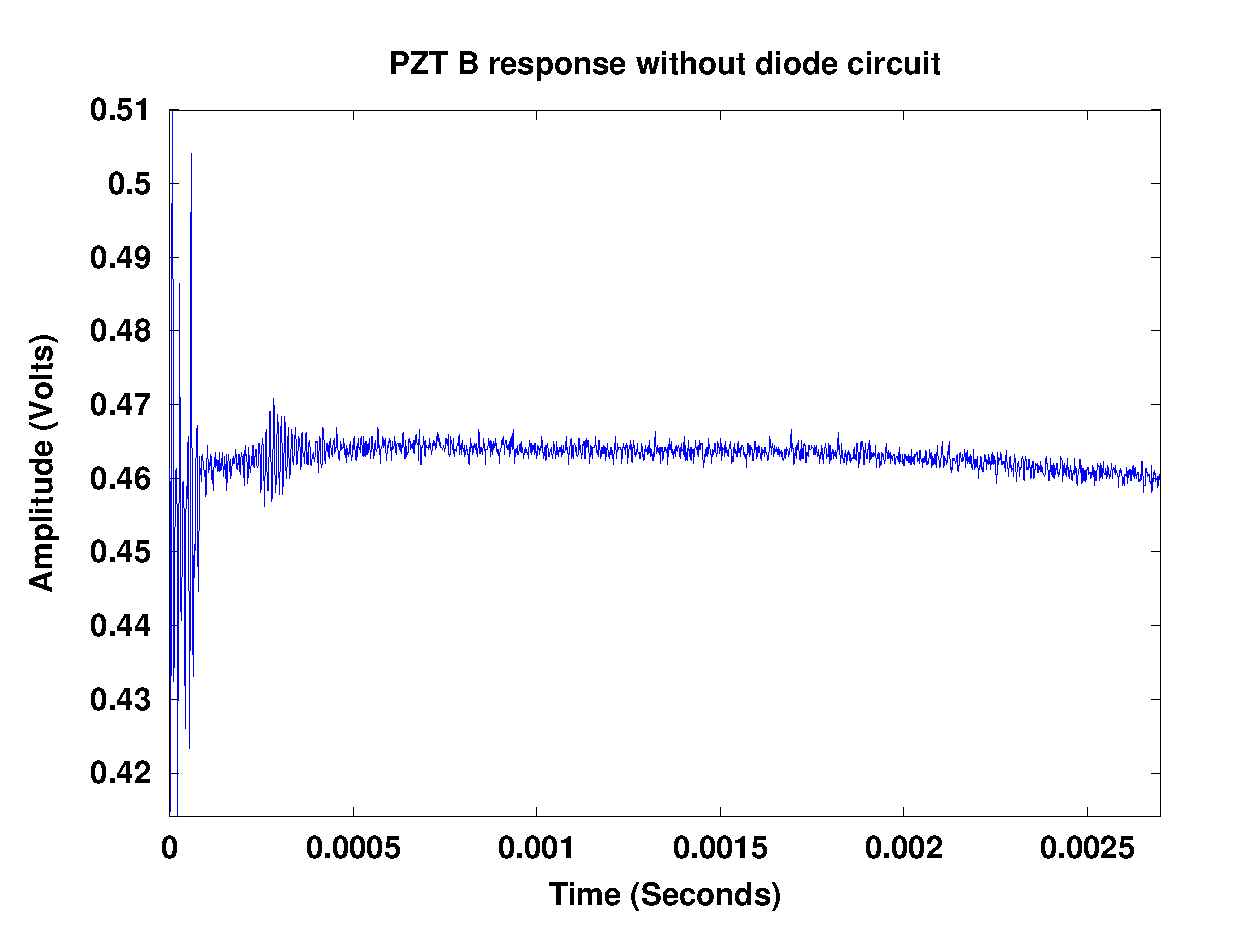
\includegraphics[width=0.6\textwidth]{eps_pics/noCircuit}}
\subfigure[Signal recorded by PZT B with the diode circuit]
{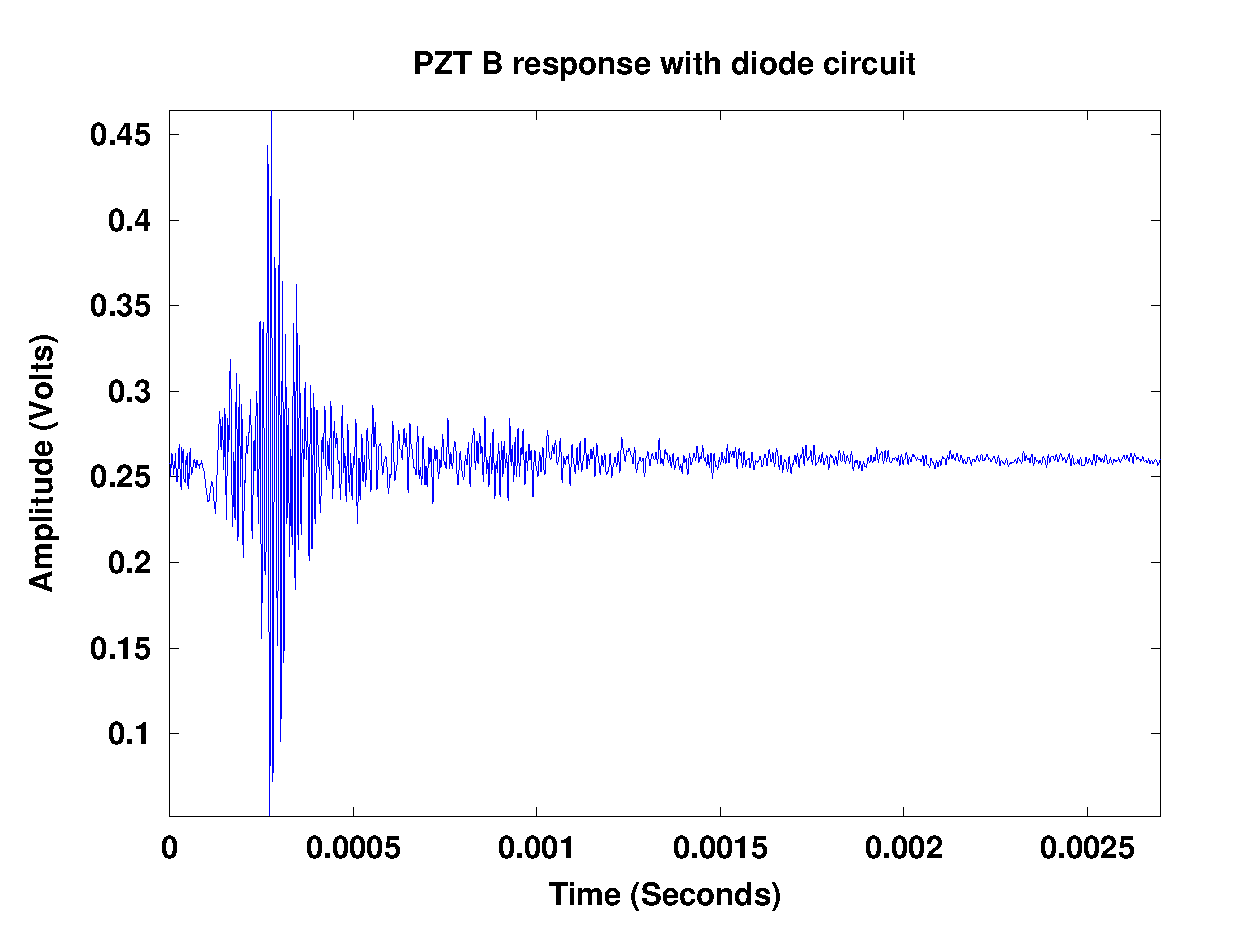
\includegraphics[width=0.6\textwidth]{eps_pics/withCircuit}}
\end{subfigmatrix}

  \caption
%>>>> use \label inside caption to get Fig. number with \ref{}
  { \label{fig:diodeCircuitResults}
(a) Signal recorded at PZT B when the diode circuit was not being used;
(b) Signal recorded at PZT B when the diode circuit was in place. It was seen that there was a large difference between the signals in (a) and (b). The wave seen in (b) was still present in (a) but was largely overshadowed by the amplifier noise.
}
\end{figure}

\section{Crack Detection Results}
The crack detection experiments were to prove that the program could detect when damage occurred within a rod. Signals were sent from PZT A and propagated through the rod where they were recorded on the other end by PZT B. The first set of tests were performed using the steel rods. The graphs of the undamaged and damaged rod tests are shown in Figure \ref{fig:steelCrackResults}. It is seen that the wave recorded by PZT B during the damaged rod tests is substantially smaller in amplitude than the wave that is recorded in the undamaged rod tests. The tests were run five times for both the undamaged and damaged samples. The signal recorded for the first test for the undamaged rod was taken to be the initial rod state. The remaining nine test signals were then compared to this first signal to determine the change in wave signature which was taken as the sum of squared differences between the signals being compared. The results from each comparison are shown in Figure \ref{fig:steelDifferences} where the damaged rod was introduced on the 6th iteration. It is seen that there was a very large jump in the computed signal difference when the damaged rod signal data was introduced. 

\begin{figure}[ht!]
\begin{subfigmatrix}{2}
\subfigure[PZT B Signal Undamaged Steel Rod]
{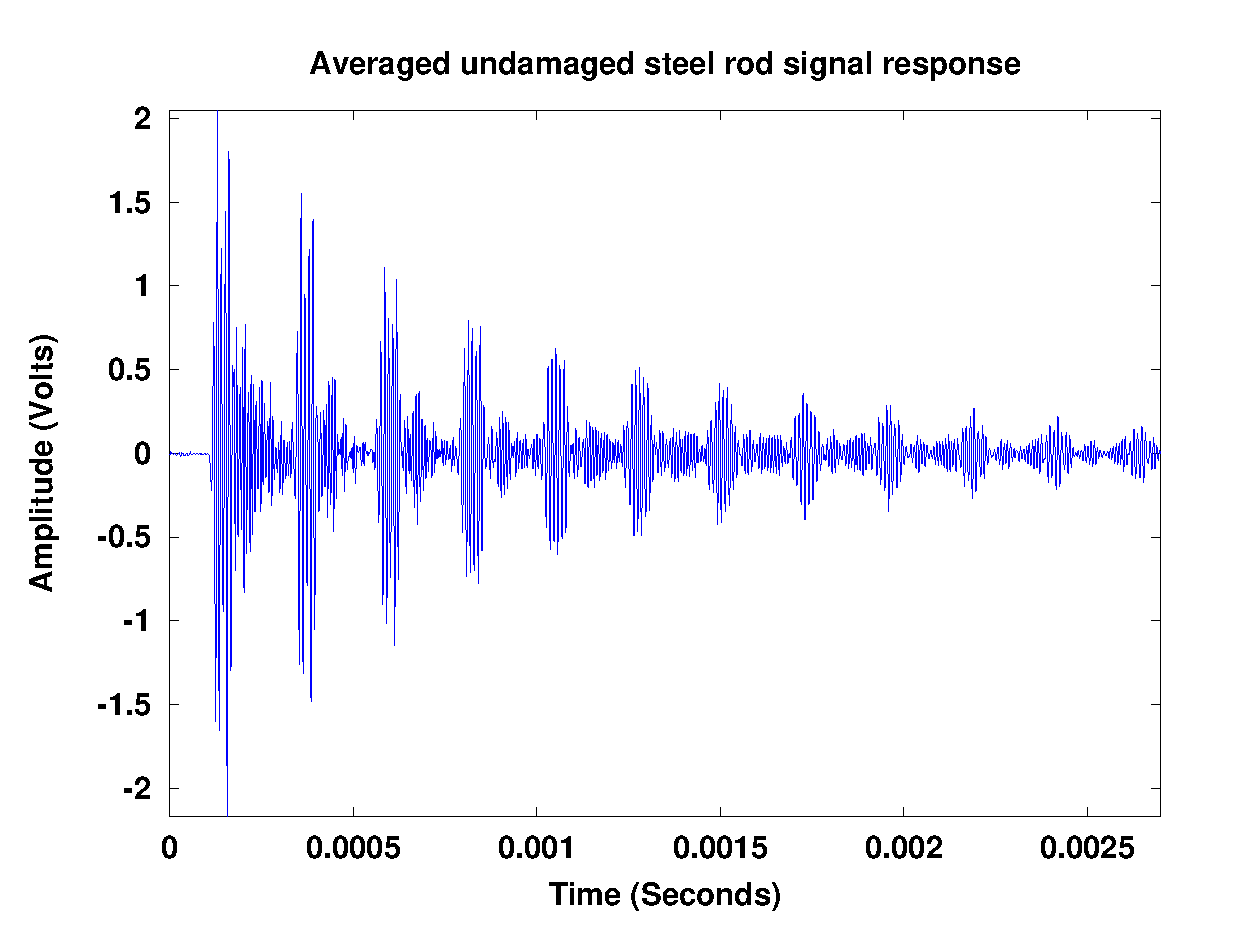
\includegraphics[width=0.6\textwidth]{eps_pics/steelUncracked}}
\subfigure[PZT B Signal Damaged Steel Rod]
{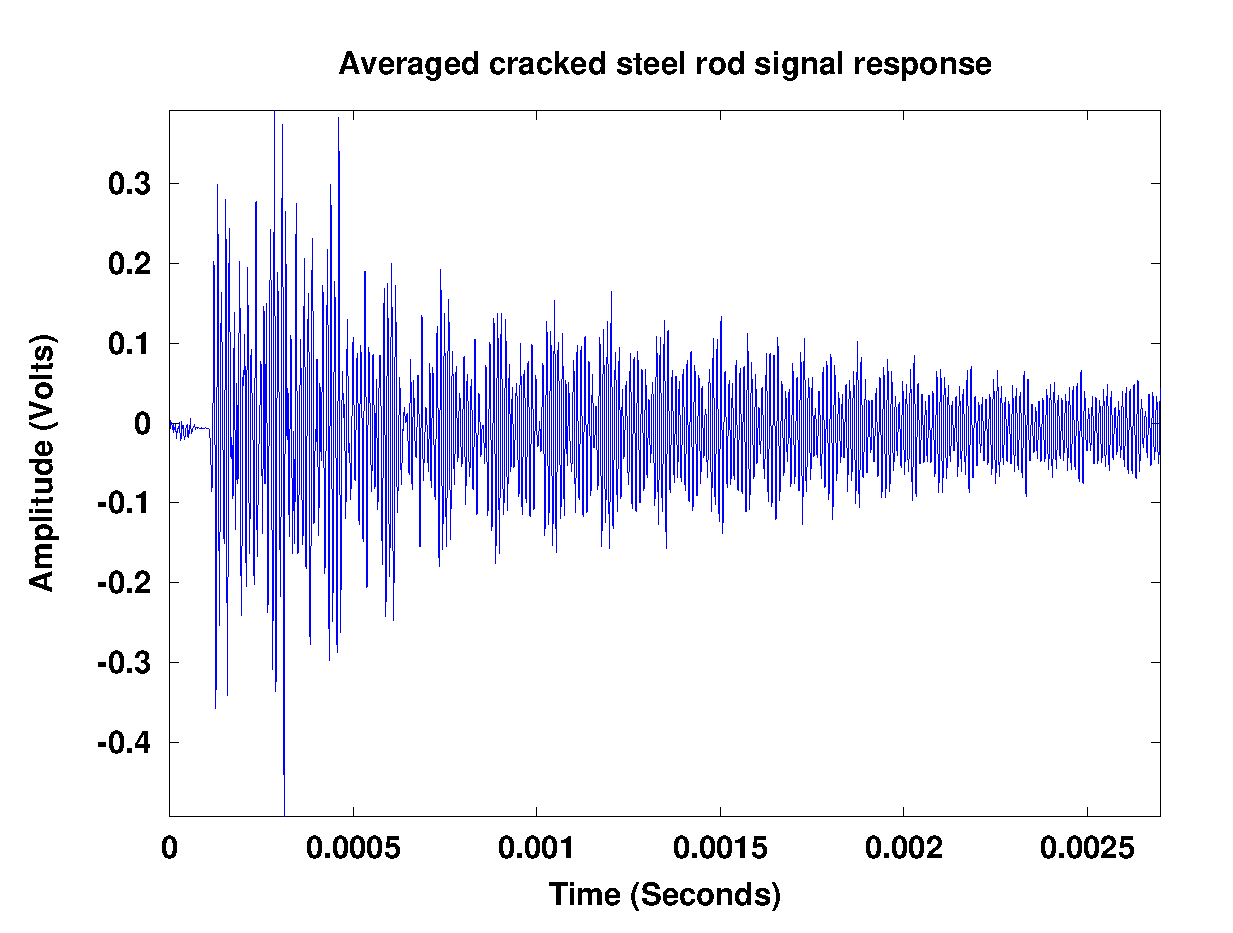
\includegraphics[width=0.6\textwidth]{eps_pics/steelCracked}}
\end{subfigmatrix}

  \caption
%>>>> use \label inside caption to get Fig. number with \ref{}
  { \label{fig:steelCrackResults}
(a) Signal recorded at PZT B with an undamaged steel rod;
(b) Signal recorded at PZT B when using the damaged nylon rod which was represented by using two rod segments whose combined length was equal to that of the undamaged rod.
}
\end{figure}

\begin{figure}[ht!]
\centering
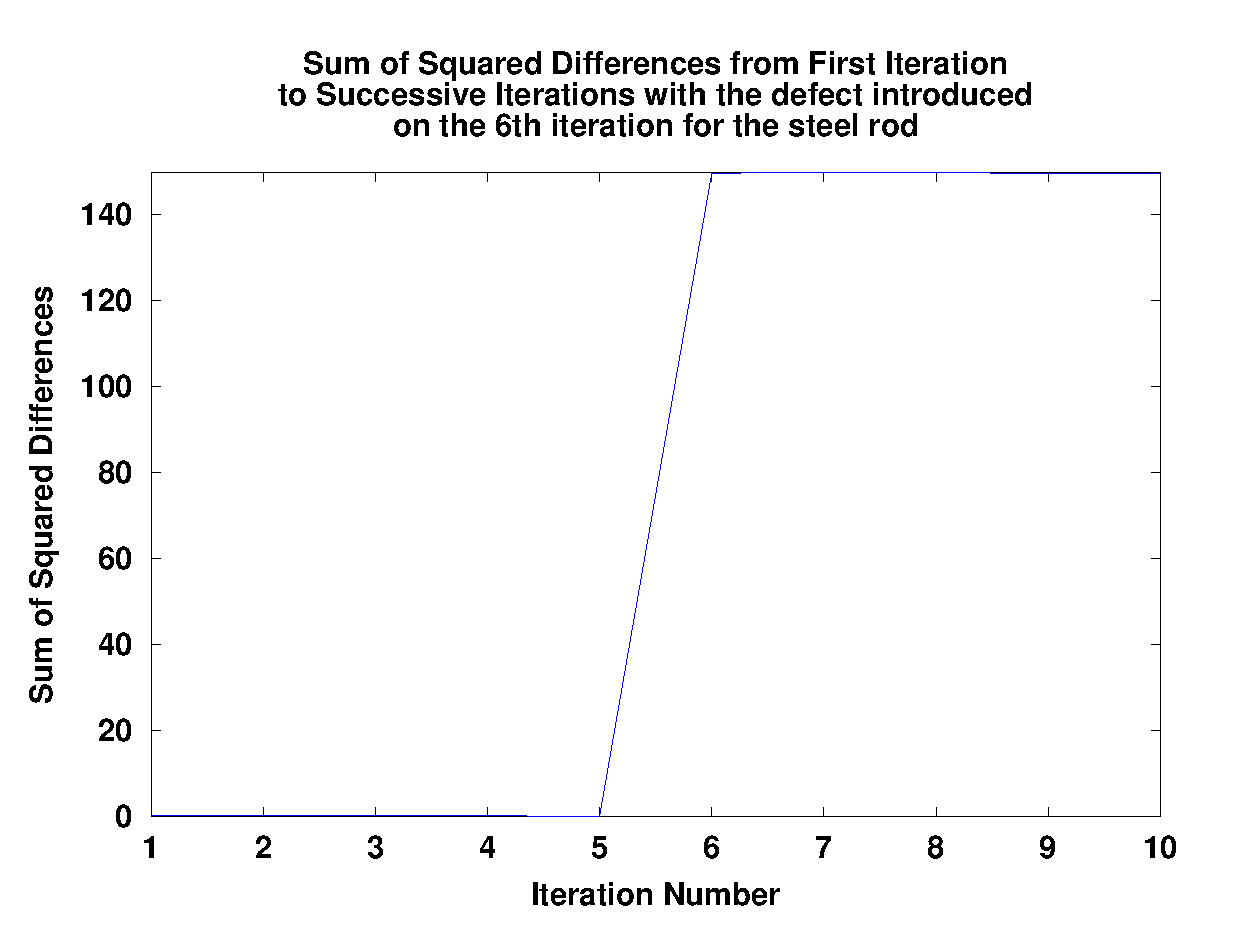
\includegraphics[width=0.6\textwidth]{eps_pics/steelDifferences}
\caption{Sum of squared differences computed for each iteration of the steel rod crack detection tests. The damaged rod was introduced on the 6th iteration and this was clearly seen in the graph data.
 	 \label{fig:steelDifferences}} 
\end{figure}

The same tests were performed using nylon rods. Figure \ref{fig:nylonCrackResults} shows the graphs for both the undamaged and damaged nylon rod crack detection tests. As with the steel rods, a large change in amplitude was seen from the undamaged to the damaged signals. Figure \ref{fig:nylonDifferences} shows the sum of squared differences for each iteration of the nylon rod tests with the damaged rod again being introduced on the 6th iteration. Just as with the steel rods a large jump in the graph was seen when the damaged rod was introduced.

\begin{figure}[ht!]
\begin{subfigmatrix}{2}
\subfigure[PZT B Signal Undamaged Nylon Rod]
{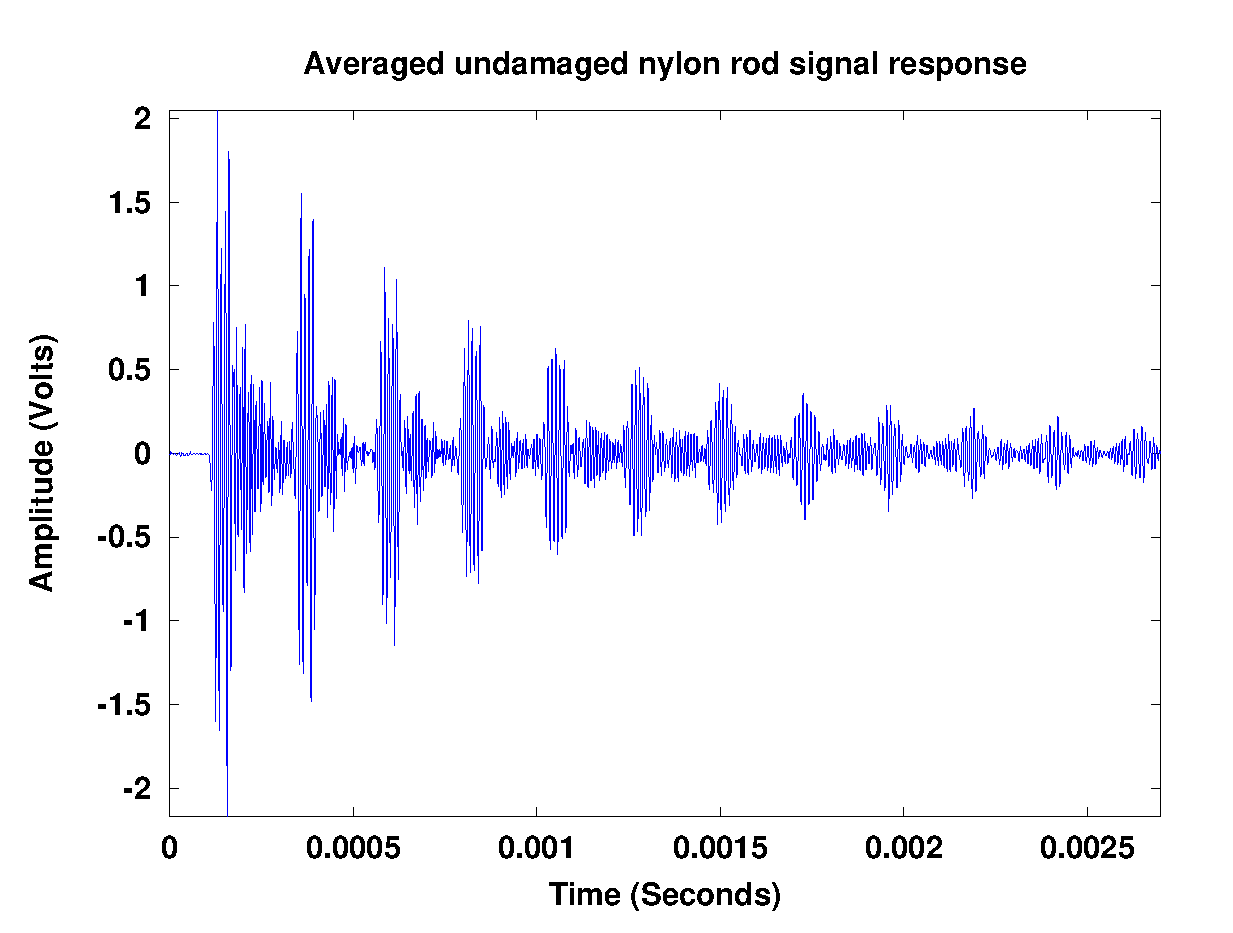
\includegraphics[width=0.6\textwidth]{eps_pics/nylonUncracked}}
\subfigure[PZT B Signal Damaged Nylon Rod]
{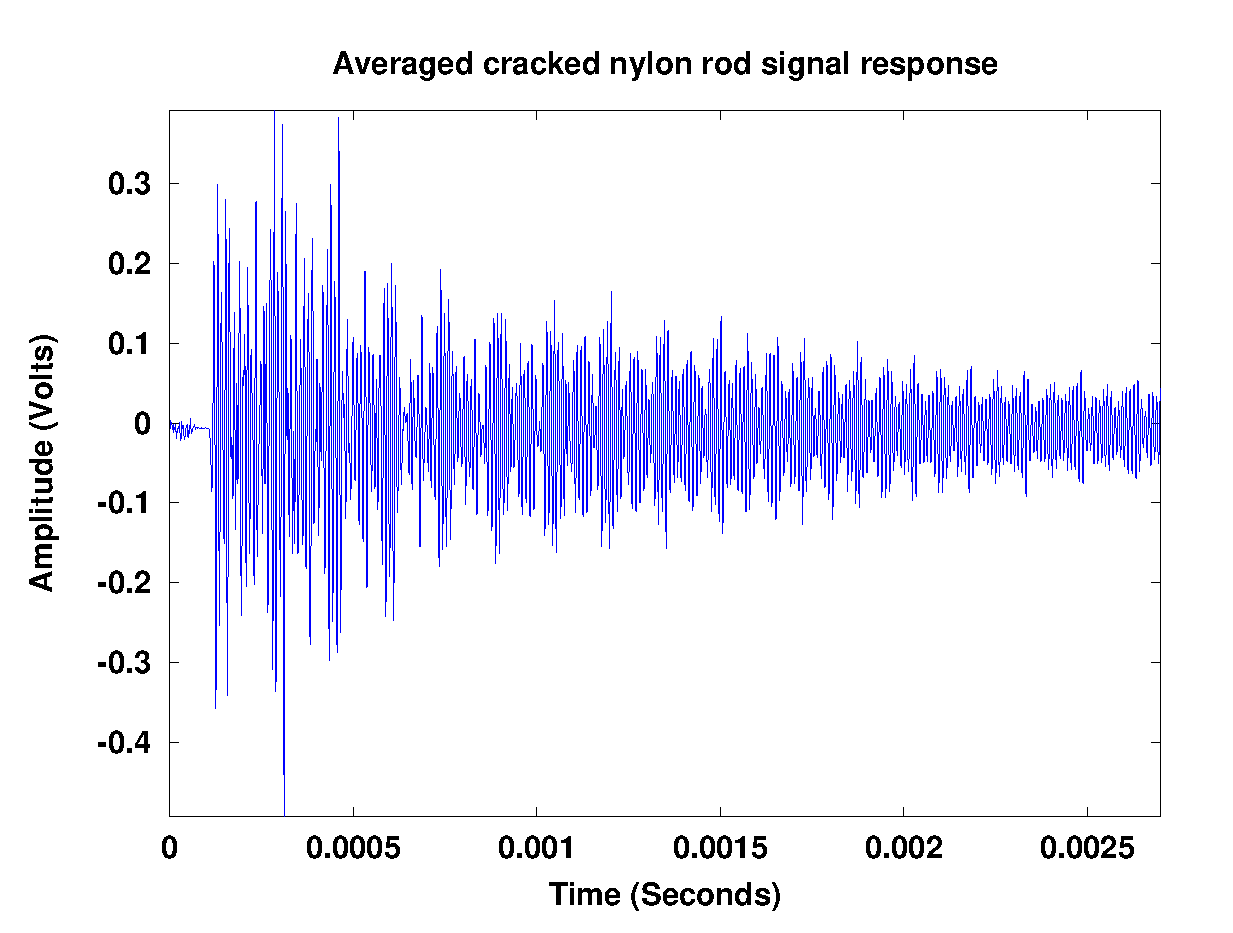
\includegraphics[width=0.6\textwidth]{eps_pics/nylonCracked}}
\end{subfigmatrix}

  \caption
%>>>> use \label inside caption to get Fig. number with \ref{}
  { \label{fig:nylonCrackResults}
(a) Signal recorded at PZT B with an undamaged nylon rod;
(b) Signal recorded at PZT B when using the damaged nylon rod which was represented by using two rod segments whose combined length was equal to that of the undamaged rod.
}
\end{figure}

\begin{figure}[ht!]
\centering
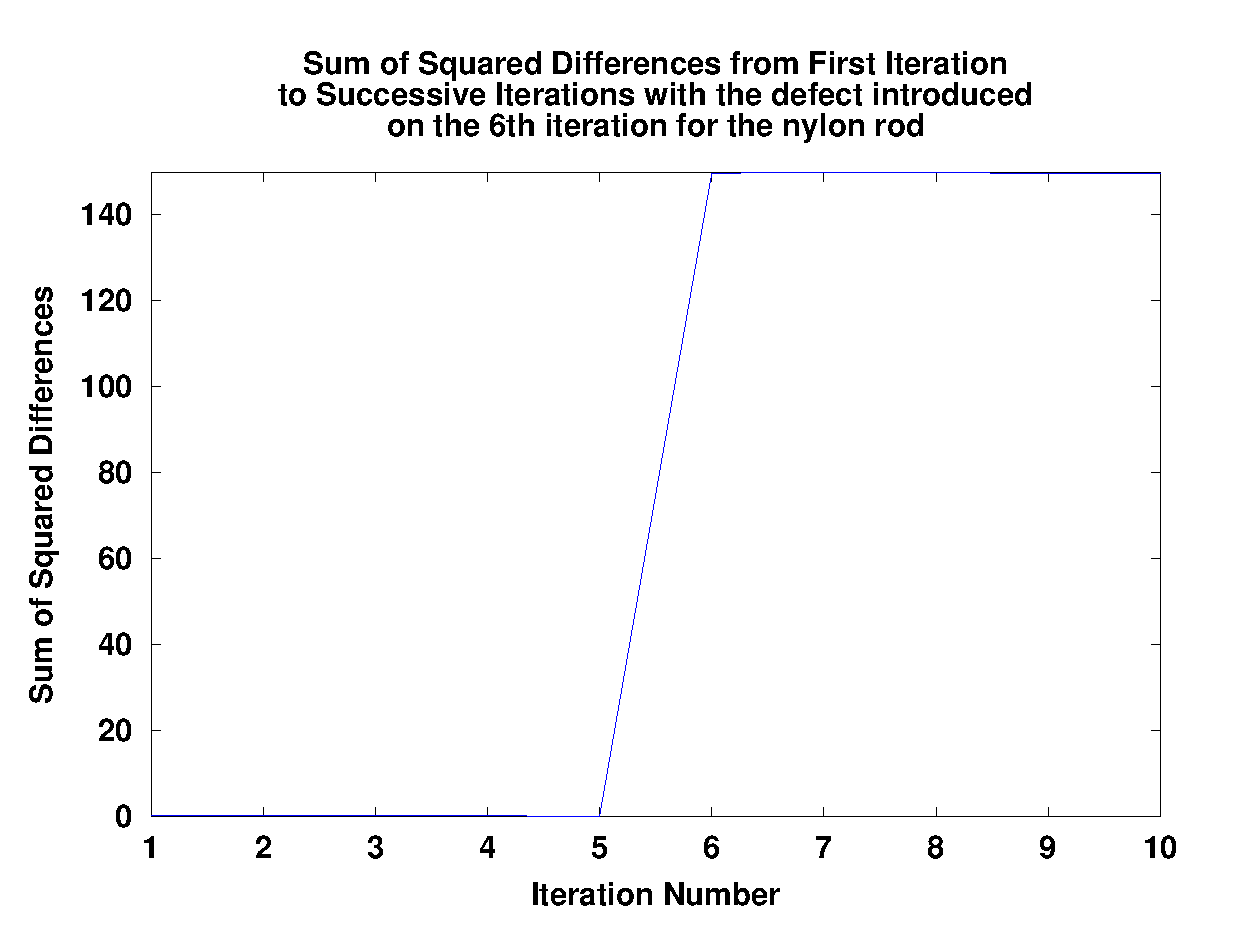
\includegraphics[width=0.6\textwidth]{eps_pics/nylonDifferences}
\caption{Sum of squared differences computed for each iteration of the nylon rod crack detection tests. The damaged rod was introduced on the 6th iteration and, as with the steel rod tests, this is clearly seen in the graph data.
 	 \label{fig:nylonDifferences}} 
\end{figure}

\section{Single Iteration Time Reversal Results}

\subsection{Steel Rods Single Iteration Results}
Theoretical calculations were carried out for the first iteration of the one dimensional time reversal focusing algorithm using the equations described in the modeling section of this thesis. Time reversal focusing was desired to be at the 'defect' PZT with a multi-tone signal over the frequency range of $100 kHz$ - $130 kHz$. The calculations were carried out assuming that there was zero dissipation. Figures \ref{fig:steelThExp1} - \ref{fig:steelThExp3} show the theoretical and experimental results together for each of the three steel rod combinations that were tested. A reasonable match between the results was seen but differences arose due to the calculations not accounting for dispersion or dissipation. The amplitude of the experimental waves are seen to have lower amplitude and an altered shape from the waves seen in the theoretical results. The wave recorded in the time reversal phase was seen to be larger than the response recorded in the interrogatory phase and was the desired result as this implied a focusing of the energy from each wave at the defect location.

\begin{figure}[ht!]
\centering
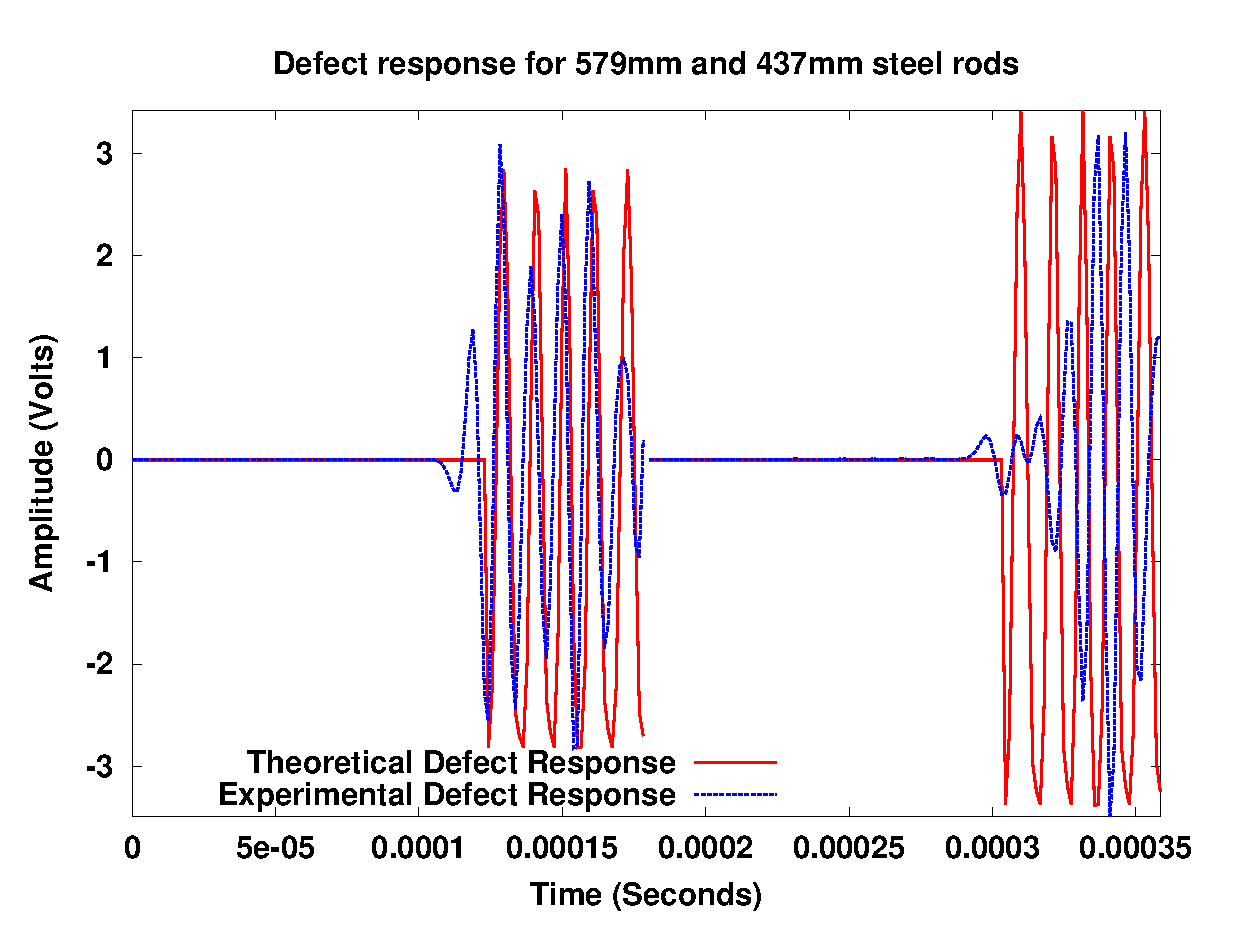
\includegraphics[width=0.6\textwidth]{eps_pics/steel-1-2_Iter_th_exp.eps}
\caption{Theory vs Experiment, $579 mm$ and $437 mm$ steel rods
	 \label{fig:steelThExp1}} 
\end{figure}

\begin{figure}[ht!]
\centering
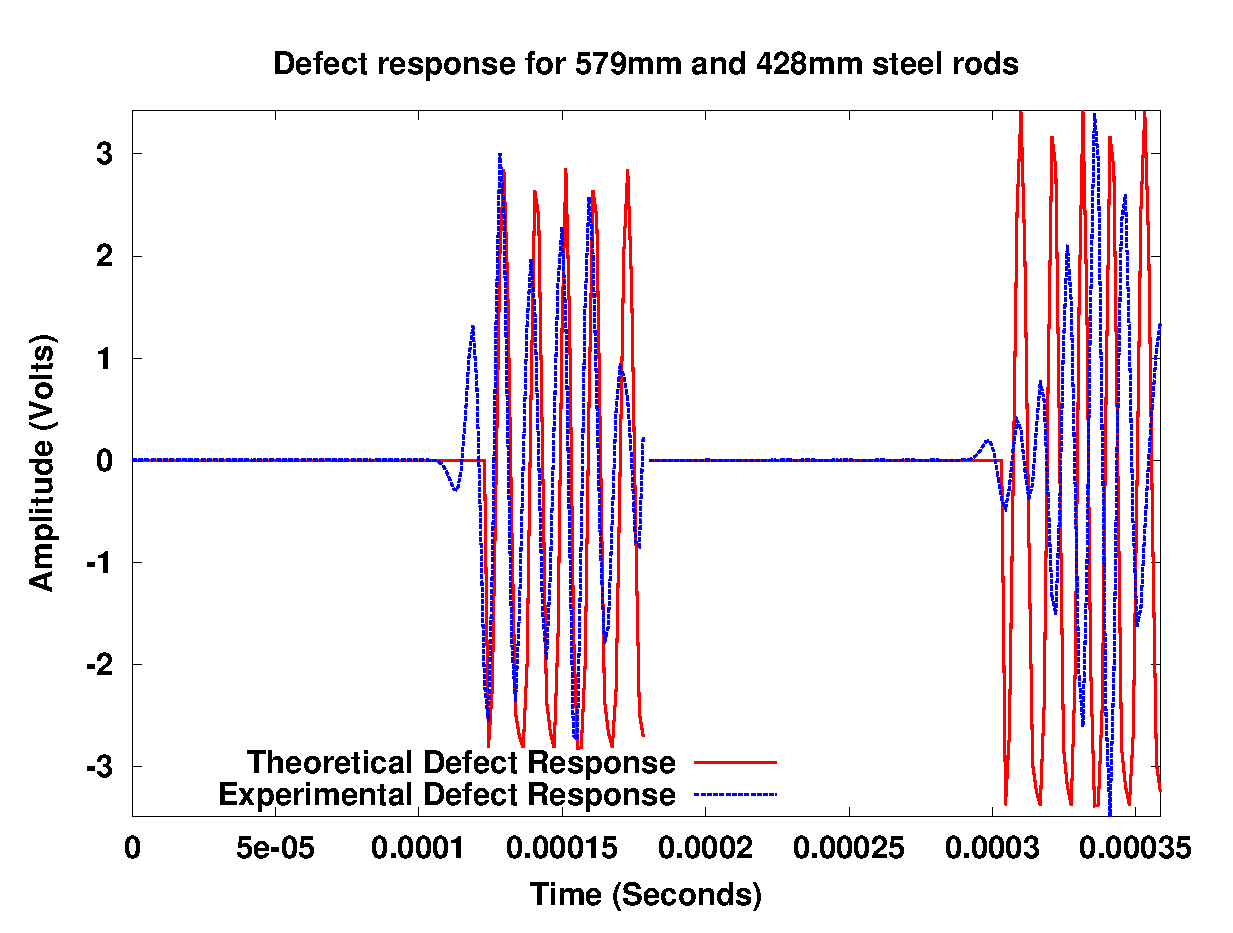
\includegraphics[width=0.6\textwidth]{eps_pics/steel-1-3_Iter_th_exp.eps}
\caption{Theory vs Experiment, $579 mm$ and $428 mm$ steel rods
	 \label{fig:steelThExp2}} 
\end{figure}

\begin{figure}[ht!]
\centering
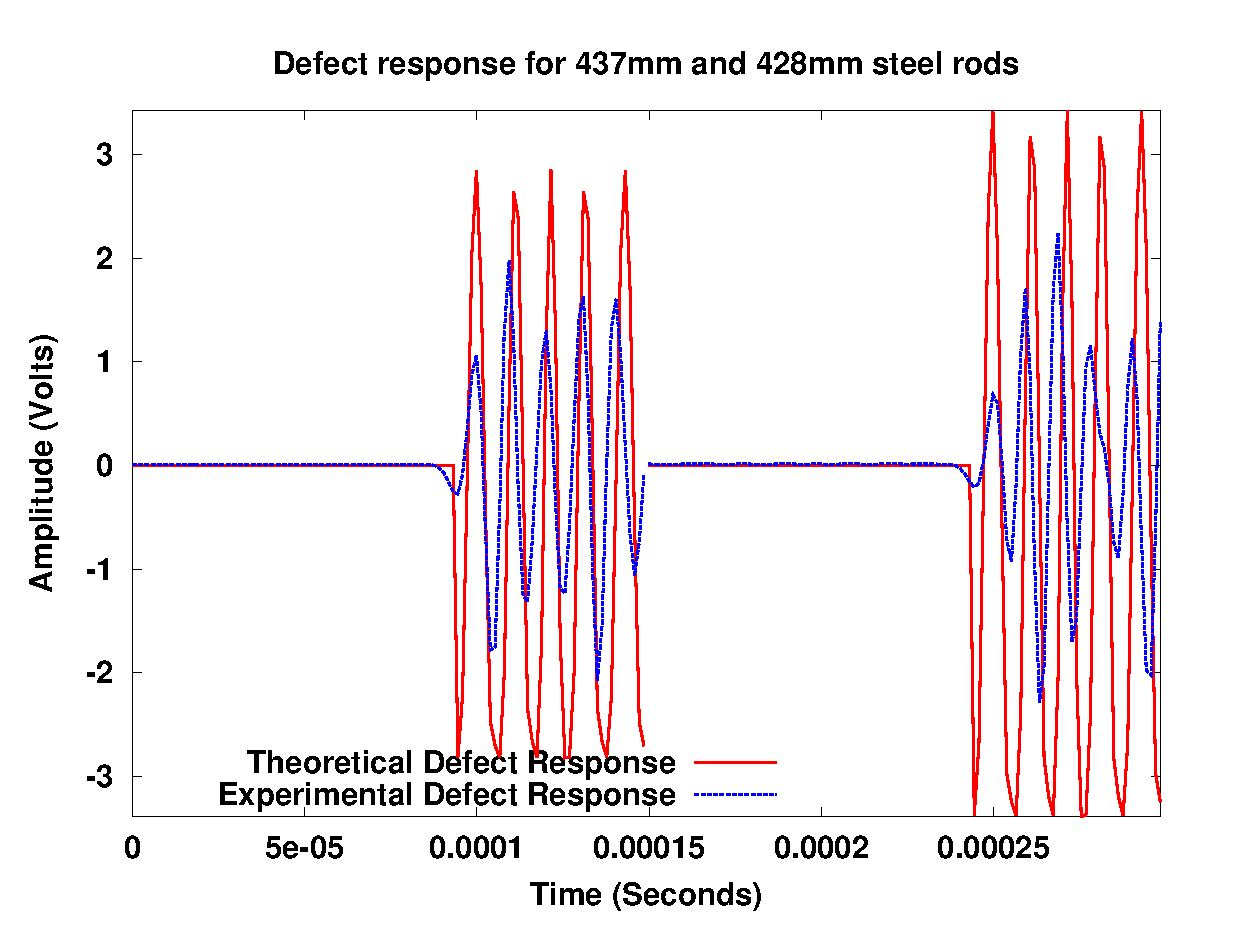
\includegraphics[width=0.6\textwidth]{eps_pics/steel-2-3_Iter_th_exp.eps}
\caption{Theory vs Experiment, $437 mm$ and $428 mm$ steel rods
	 \label{fig:steelThExp3}} 
\end{figure}

 \subsection{Nylon Rods Single Iteration Results}
 Calculations were carried out for the nylon rods which were also based upon the models seen previously in this paper. The calculations for the nylon rods also ignored dispersion and dissipation. As with the steel rods, these theoretical results were compared with the experimental results and this comparison is shown for each of the three nylon rod tests Figures \ref{fig:nylonThExp1} - \ref{fig:nylonThExp3}. A worse match was seen in these experiments and was perhaps due to greater dispersion and dissipation within the nylon rods than seen in the steel rods. The overall result was still good though because the wave in the time reversal phase wass again seen to be larger than the wave recorded in the interrogatory phase. This increase in amplitude showed that focusing occurred with the nylon rod tests. 
 
 \begin{figure}[ht!]
 \centering
 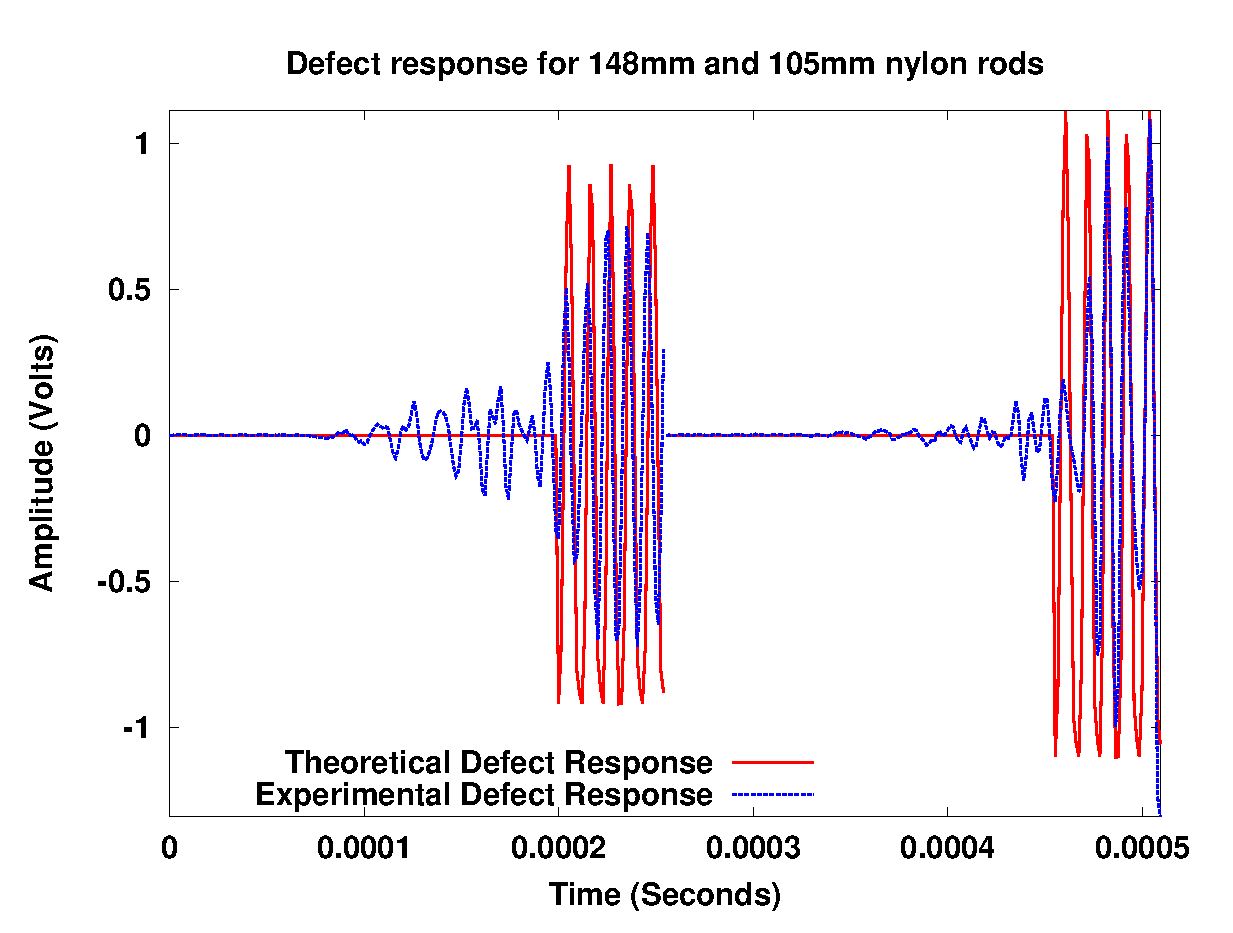
\includegraphics[width=0.6\textwidth]{eps_pics/nylon-2-3_Iter_th_exp.eps}
 \caption{Theory vs Experiment, $148 mm$ and $105 mm$ nylon rods
 	 \label{fig:nylonThExp1}} 
 \end{figure}
 
 \begin{figure}[ht!]
 \centering
 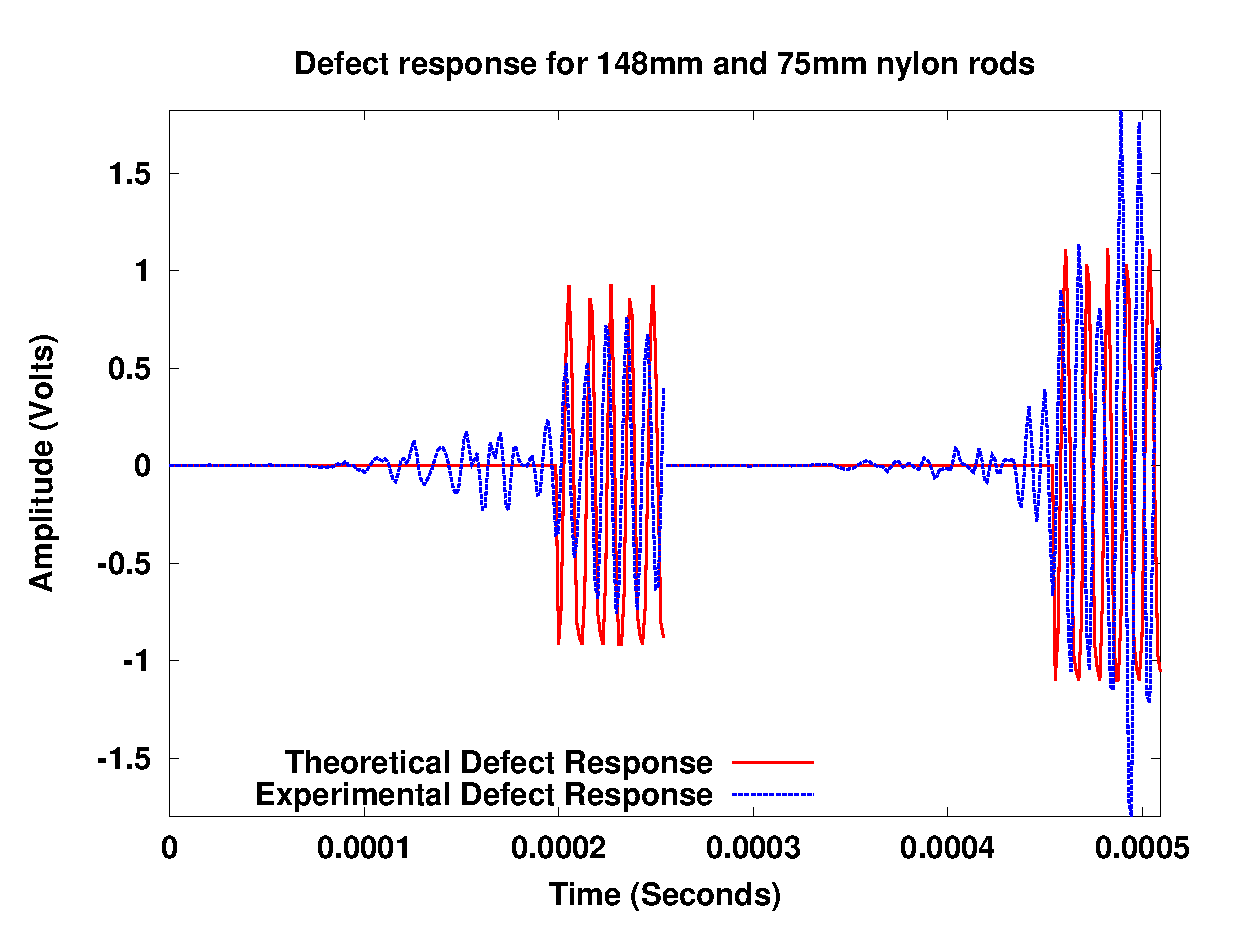
\includegraphics[width=0.6\textwidth]{eps_pics/nylon-2-4_Iter_th_exp.eps}
 \caption{Theory vs Experiment, $148 mm$ and $75 mm$ nylon rods
 	 \label{fig:nylonThExp2}} 
 \end{figure}
 
 \begin{figure}[ht!]
 \centering
 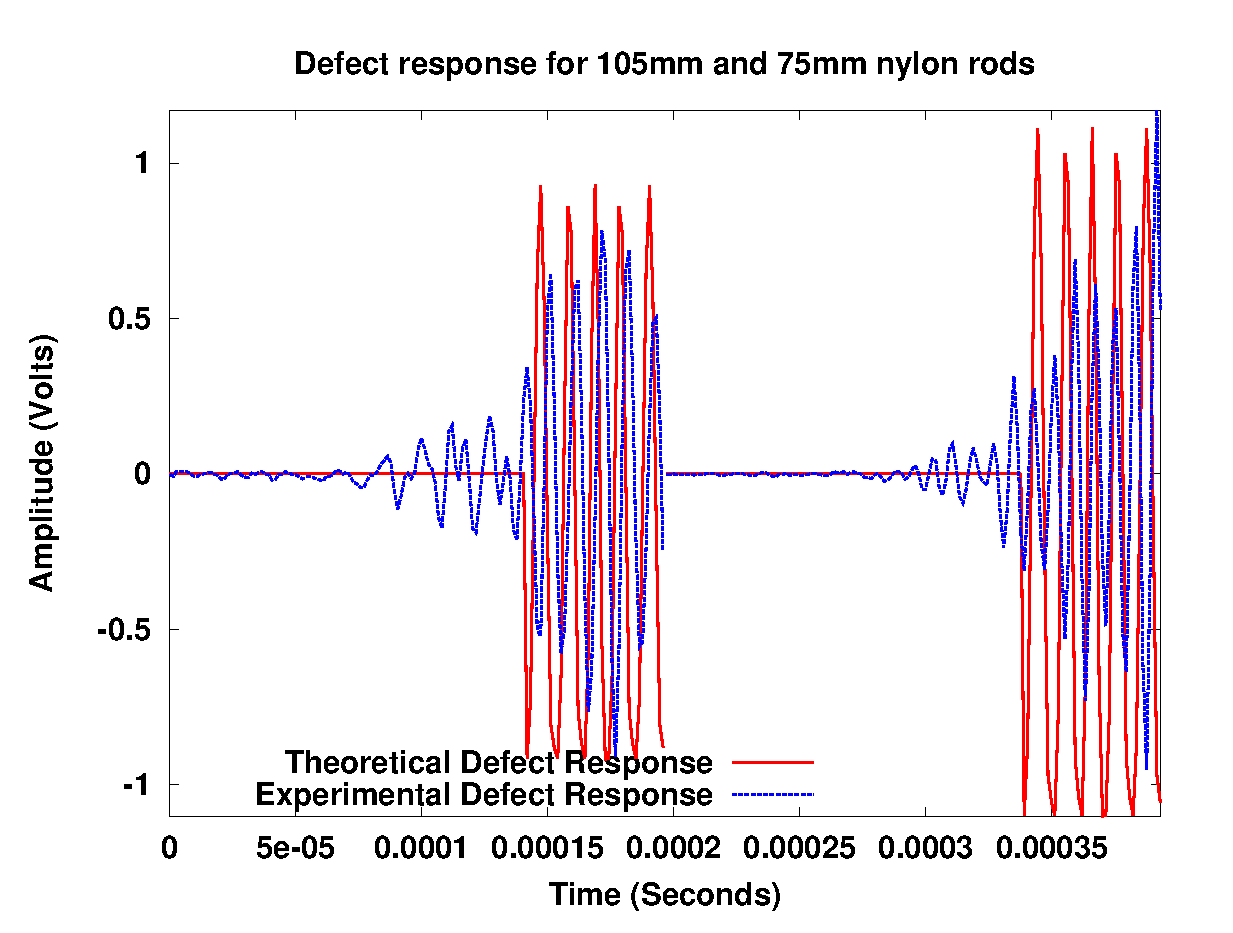
\includegraphics[width=0.6\textwidth]{eps_pics/nylon-3-4_Iter_th_exp.eps}
 \caption{Theory vs Experiment, $105 mm$ and $75 mm$ nylon rods
 	 \label{fig:nylonThExp3}} 
 \end{figure}
 
 
 \section{Iterative Time Reversal Results}
 The time reversal algorithm was applied iteratively in both the steel and nylon rod tests. The goal of the iterative reversal was to see an increase in the response amplitude at the defect with each iteration. For each iteration the amplitude gain at the defect was recorded and used to determine the overall effectiveness of applying the time  reversal algorithm in an iterative fashion. The gain was determined by comparing the max peak to peak amplitude recorded at the defect on each iteration with the max response recorded on the first iteration. The max peak to peak amplitude was taken to be $|max(DefectVoltage) - min(DefectVOltage)|$. The gain was then computed as $CurrentMax / InitialMax$ and this was plotted for each time reversal iteration. 
 
 \subsection{Steel Rods Multiple Iteration Results}
 For the steel rod tests it was seen that the amplitude of the gain increased rapidly in the beginning of the experiments as the algorithm found a better and better signal with each iteration for the PZTs to playback. The gain began to level off as the number of iterations increased and the algorithm started to converge on a playback signal for each PZT. In the gain plots for the three steel rod tests it was seen that the gain increased substantially in the beginning and then leveled out (Figures \ref{fig:steelIter1} - \ref{fig:steelIter3}). It was noticed that the final gain seen may not necessarily have been the maximum gain achieved throughout the iterative process. This suggests that further refinements could be made to the time reversal algorithm such that the optimal playback waves would be found, and also suggests that more descriptive models are needed to further understand the underlying principles of time reversal.

\begin{figure}[ht!]
\centering
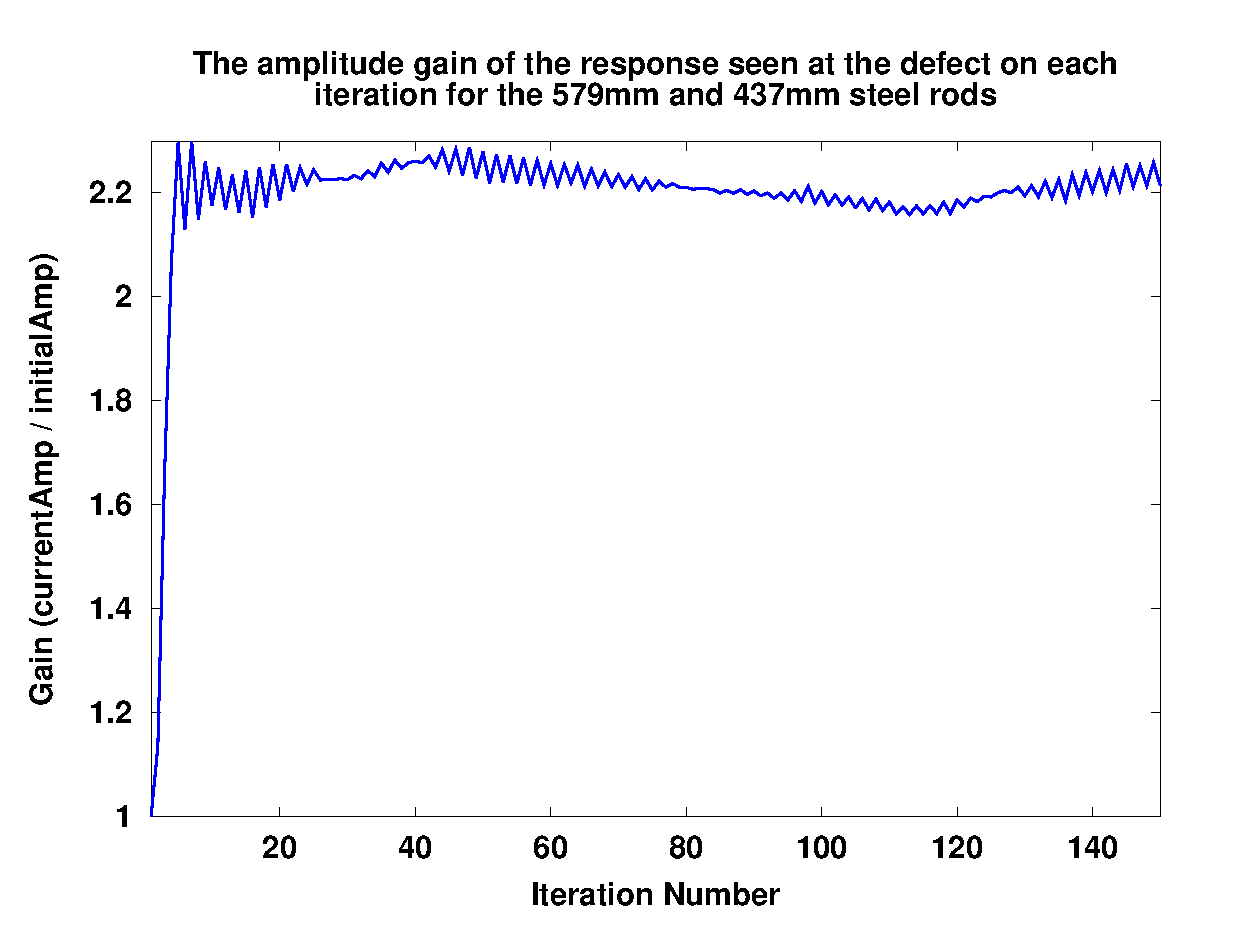
\includegraphics[width=0.6\textwidth]{eps_pics/steel-1-2_iterationVsGain.eps}
\caption{Amplitude gain at the defect on each iteration for the $579 mm$ and $437 mm$ steel rod iterative time reversal test with a final gain of a little over 2. The gain did not appear to completely level out, but it slowly oscillated right around 2.
	 \label{fig:steelIter1}} 
\end{figure}
  
\begin{figure}[ht!]
\centering
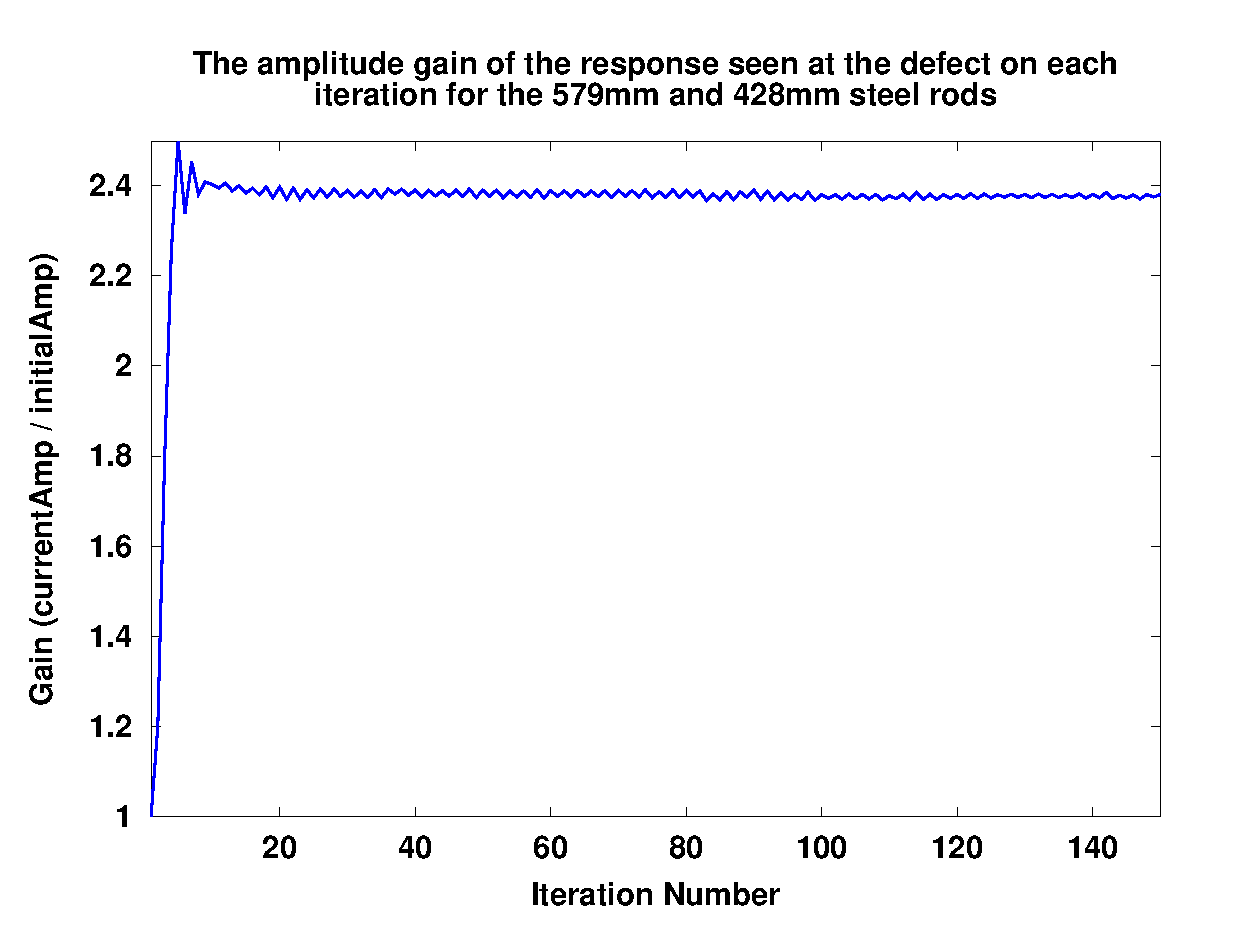
\includegraphics[width=0.6\textwidth]{eps_pics/steel-1-3_iterationVsGain.eps}
\caption{Defect amplitude gain on each iteration for the $579 mm$ and $428 mm$ steel rod iterative time reversal test with a final gain of a little over 2.5.
 	 \label{fig:steelIter2}} 
\end{figure}

\begin{figure}[ht!]
\centering
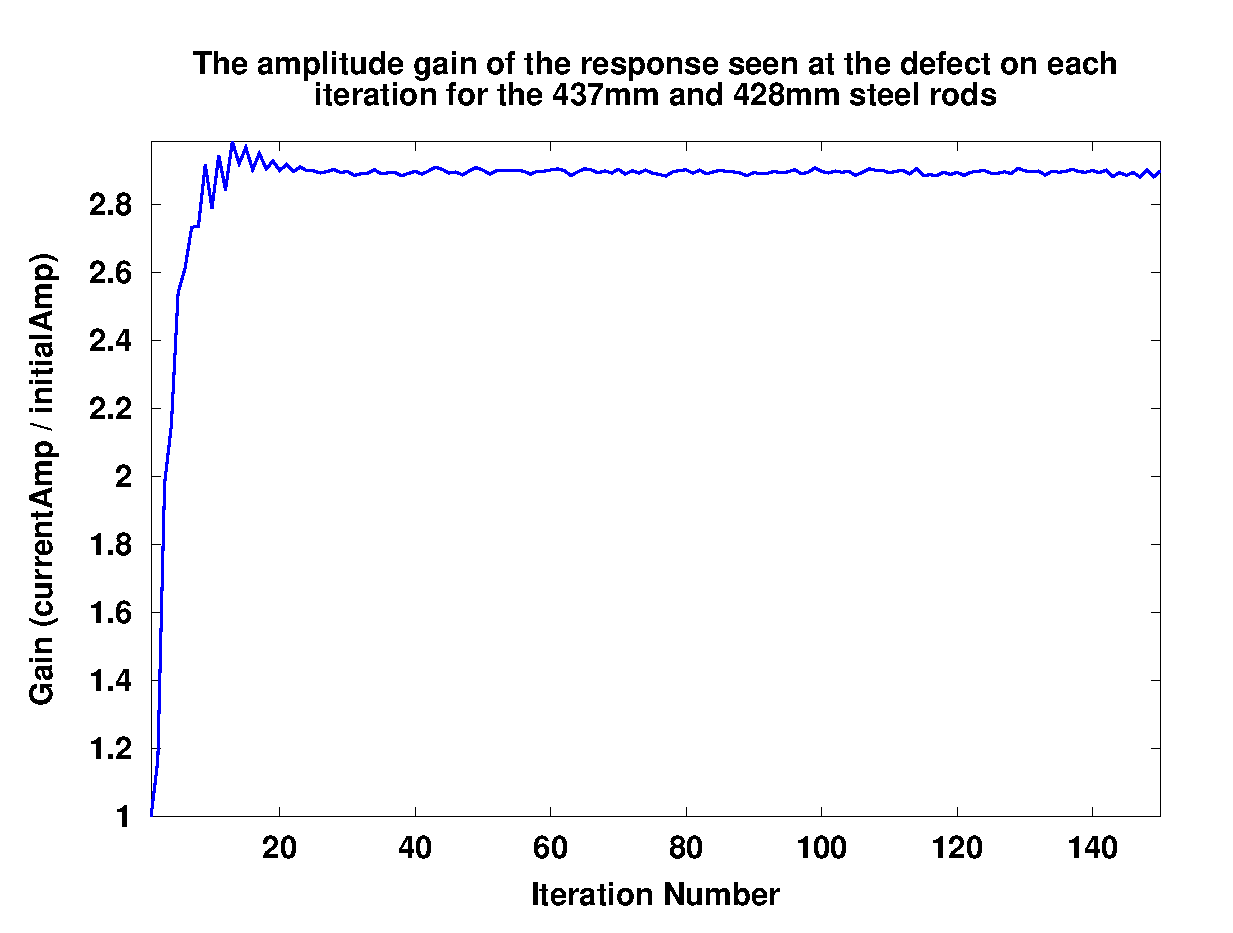
\includegraphics[width=0.6\textwidth]{eps_pics/steel-2-3_iterationVsGain.eps}
\caption{Defect amplitude gain on each iteration for the $437 mm$ and $428 mm$ steel rod iterative time reversal test with a final gain of about 3.
  	 \label{fig:steelIter3}} 
\end{figure}

 
 The other method used to gauge the performance of the iterative time reversal was to compare the signature of the response at the defect on both the first and last iteration. If the algorithm worked correctly then what should have been seen is that the final wave was purer and of larger amplitude than the initial wave. This is in fact what was seen in the steel rod tests. The comparison of the first and initial waves at the defect are shown for each of the three steel rod tests in Figures \ref{fig:steelExp1} - \ref{fig:steelExp3}.
 
  \begin{figure}
 \begin{subfigmatrix}{2}
 \subfigure[Defect Response Initial Iteration, $579 mm$ and $437 mm$ steel rods]
 {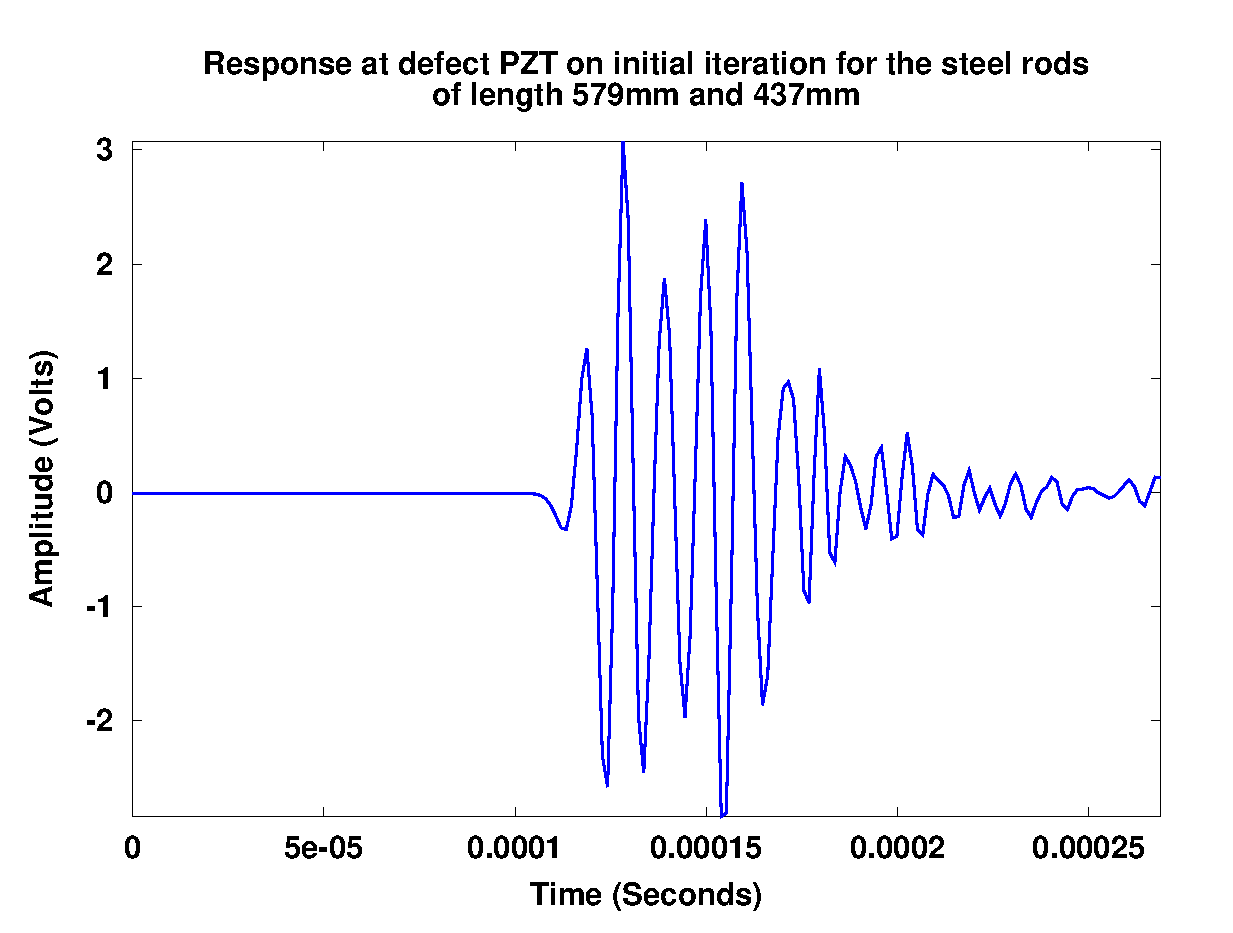
\includegraphics[width=0.6\textwidth]{eps_pics/steel-1-2_Initial.eps}}
 \subfigure[Defect Response 150th Iteration, $579 mm$ and $437 mm$ steel rods]
 {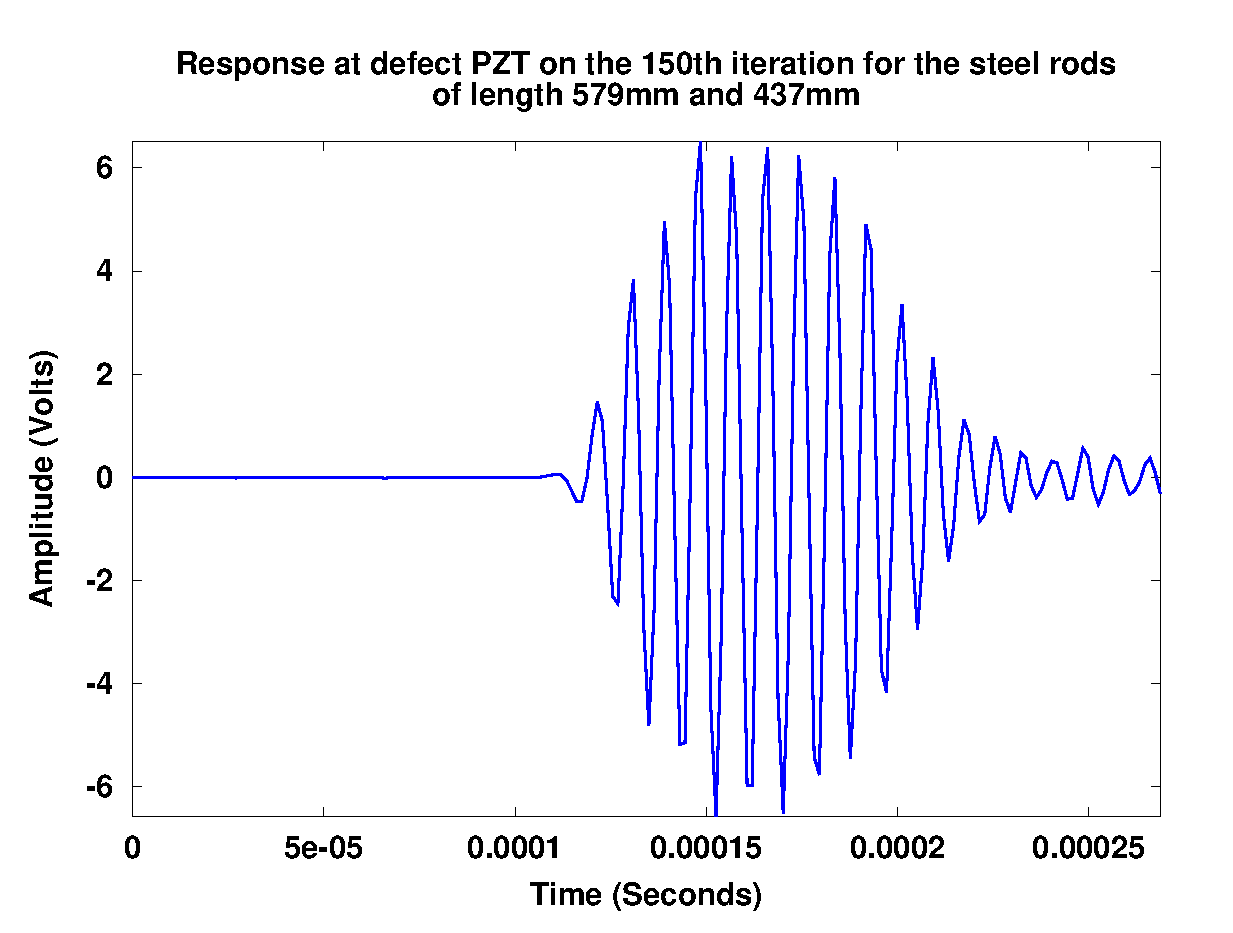
\includegraphics[width=0.6\textwidth]{eps_pics/steel-1-2_Final.eps}}
 \end{subfigmatrix}
 
    \caption
 %>>>> use \label inside caption to get Fig. number with \ref{}
    { \label{fig:steelExp1}
    a) First wave seen at the defect on the initial iteration for the $579 mm$ and $437 mm$ steel rod test.; b) Wave recorded at the defect after 150 iterations. The wave was much more defined and more than doubled in amplitude since the first iteration.
  }
 \end{figure}
 
  \begin{figure}
 \begin{subfigmatrix}{2}
 \subfigure[Defect Response Initial Iteration, $579 mm$ and $428 mm$ steel rods]
 {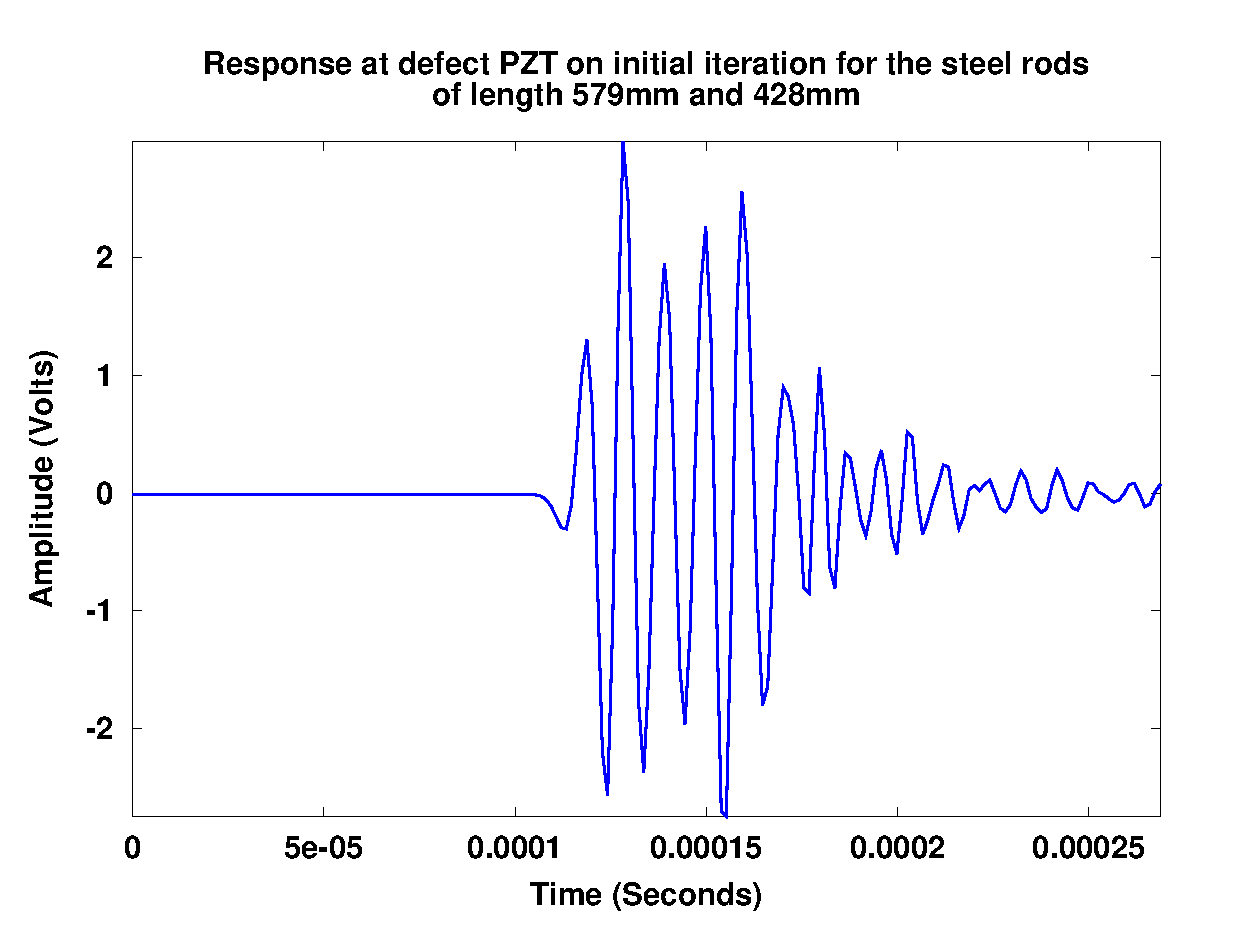
\includegraphics[width=0.6\textwidth]{eps_pics/steel-1-3_Initial.eps}}
 \subfigure[Defect Response 150th Iteration, $579 mm$ and $428 mm$ steel rods]
 {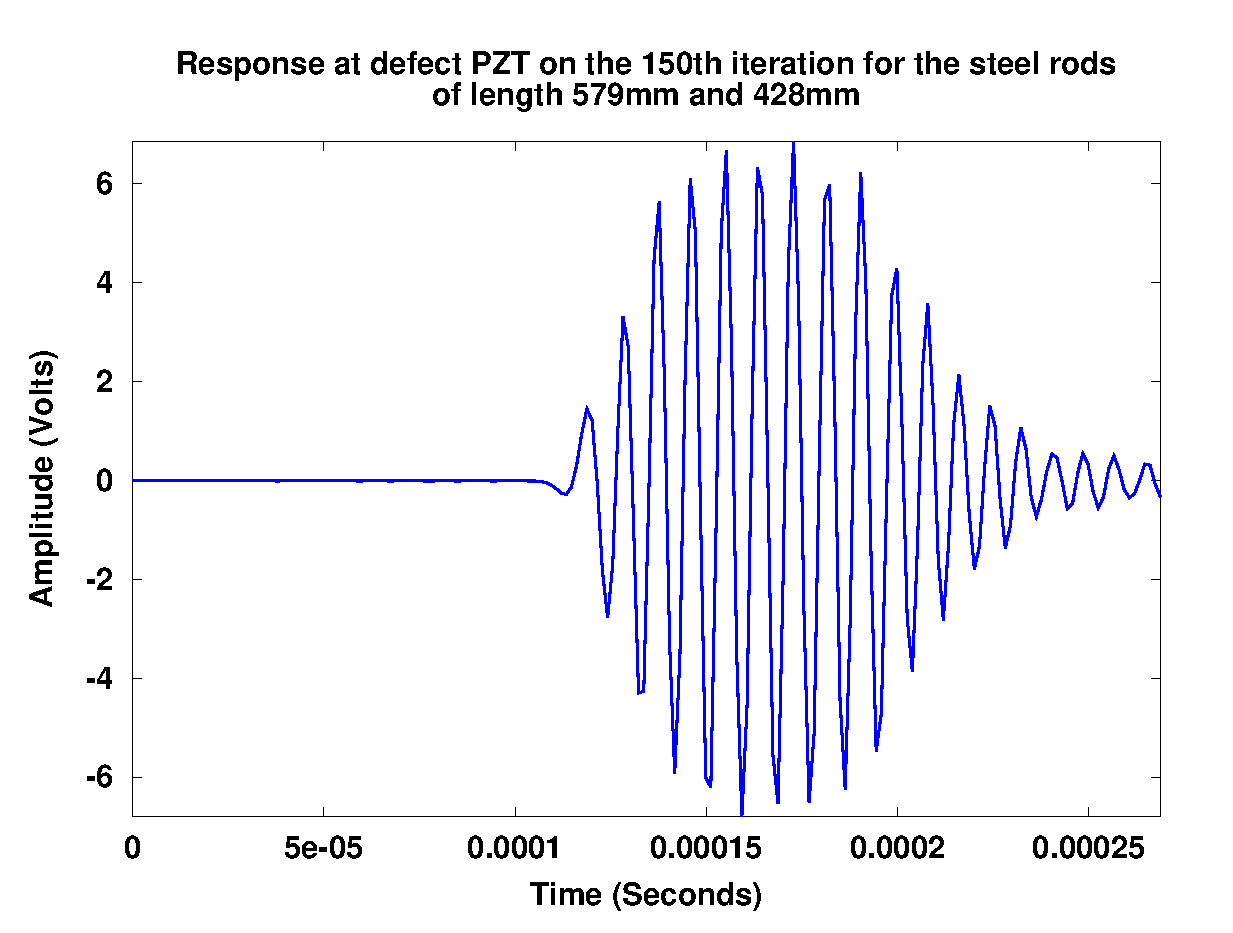
\includegraphics[width=0.6\textwidth]{eps_pics/steel-1-3_Final.eps}}
 \end{subfigmatrix}
 
    \caption
 %>>>> use \label inside caption to get Fig. number with \ref{}
    { \label{fig:steelExp2}
    a) First wave seen at the defect on the initial iteration for the $579 mm$ and $428 mm$ steel rod test.; b) Wave recorded at the defect after 150 iterations. Like the $579 mm$ and $437 mm$ steel rod results, this wave was much more defined and more than doubled in amplitude since the first iteration.
  }
 \end{figure}
 
  \begin{figure}
 \begin{subfigmatrix}{2}
 \subfigure[Defect Response Initial Iteration, $437 mm$ and $428 mm$ steel rods]
 {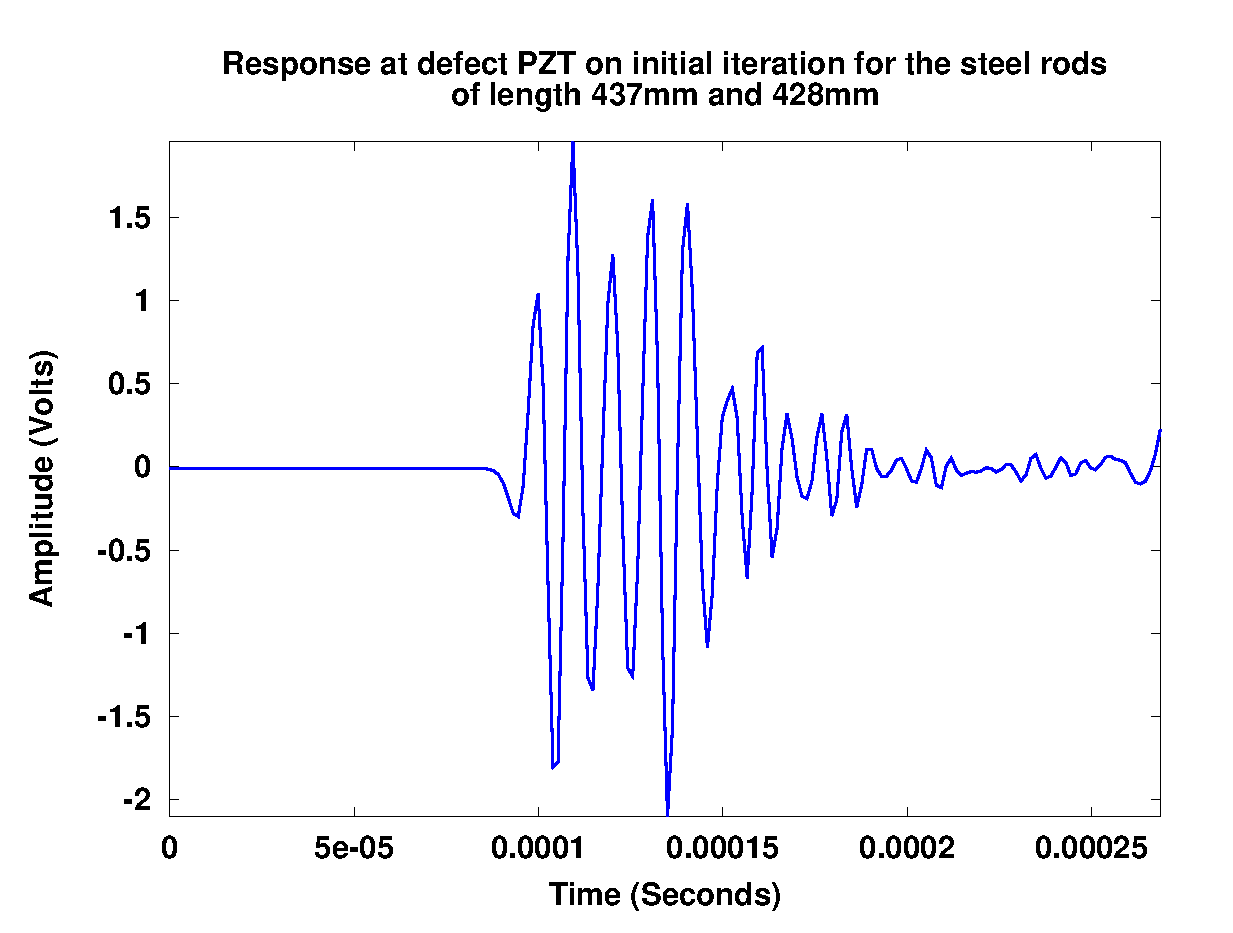
\includegraphics[width=0.6\textwidth]{eps_pics/steel-2-3_Initial.eps}}
 \subfigure[Defect Response 150th Iteration, $437 mm$ and $428 mm$ steel rods]
 {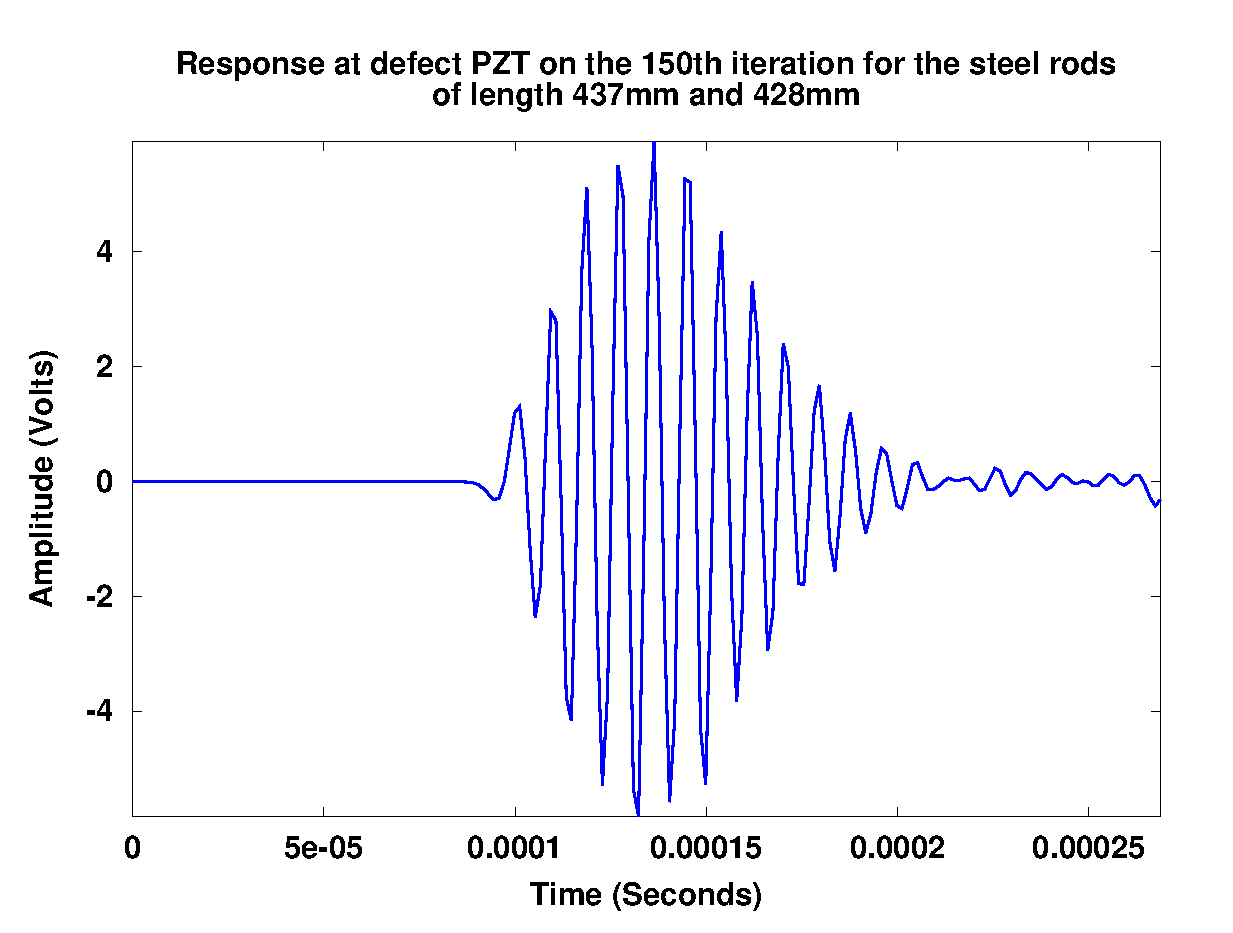
\includegraphics[width=0.6\textwidth]{eps_pics/steel-2-3_Final.eps}}
 \end{subfigmatrix}
 
    \caption
 %>>>> use \label inside caption to get Fig. number with \ref{}
    { \label{fig:steelExp3}
    a) First wave seen at the defect on the initial iteration for the $437 mm$ and $428 mm$ steel rod test.; b) Wave recorded at the defect after 150 iterations. The amplitude of the wave nearly tripled since the first iteration.
  }
 \end{figure}
 
 \subsection{Nylon Rods Multiple Iteration Results}
 As with the steel rod tests, the amplitude gain seen at the defect on each iteration was plotted for the three nylon rod tests (Figures \ref{fig:nylonIter1} - \ref{fig:nylonIter2}). With the nylon rods an even higher gain was seen than with the steel rod tests. The nylon tests showed an average gain of over 3 whereas the gains seen with the steel rod tests were closer to 2. The first and final waves recorded at the defect are also compared for each of the nylon tests and these results are shown in Figures \ref{fig:nylonExp1} - \ref{fig:nylonExp3}. It was seen that final wave was of much greater amplitude than the initial wave for all of the tests performed.
 
 \begin{figure}[ht!]
 \centering
 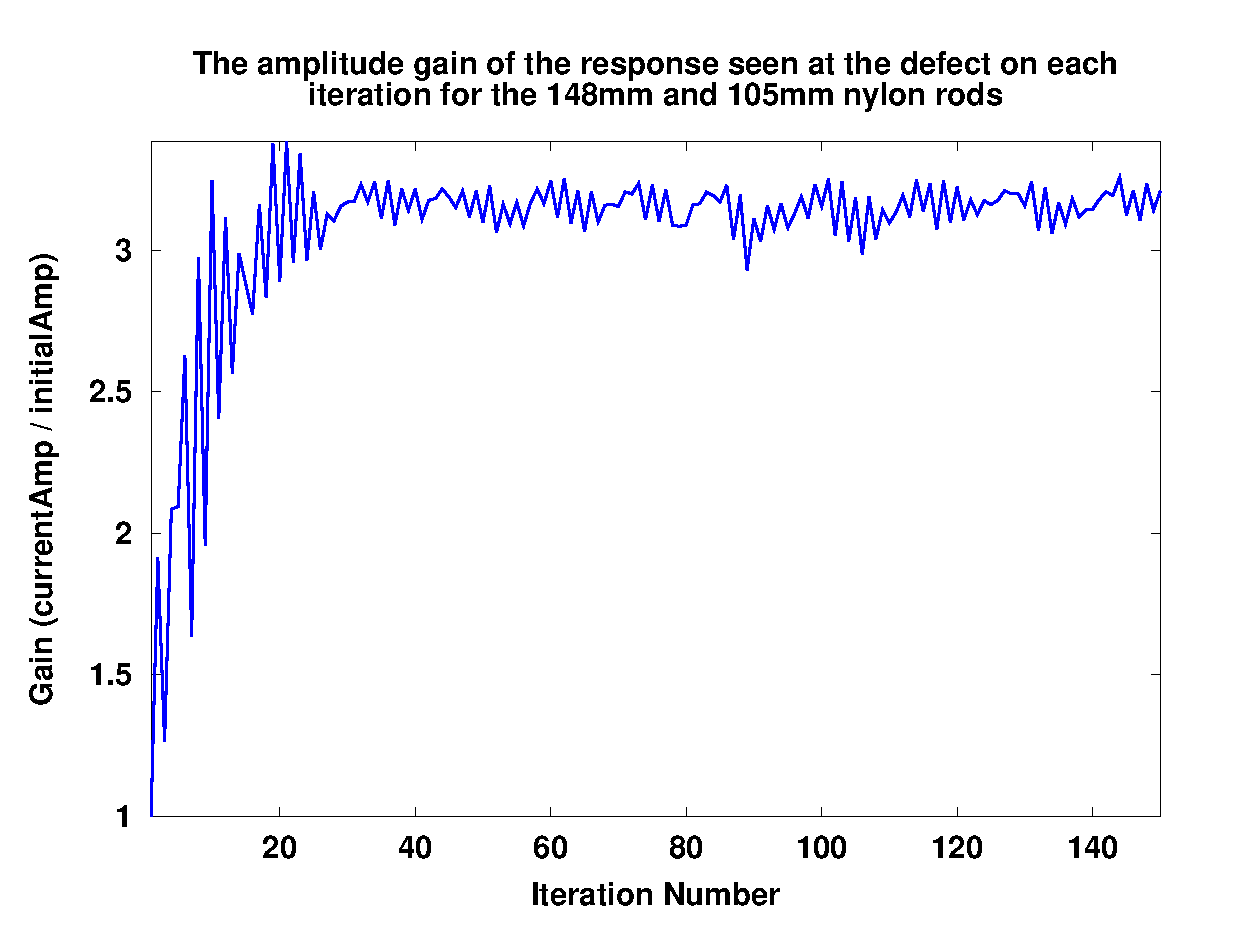
\includegraphics[width=0.6\textwidth]{eps_pics/nylon-2-3_iterationVsGain.eps}
 \caption{Defect amplitude gain that was achieved at the defect for each iteration of the time reversal algorithm for the $148 mm$ and $105 mm$ nylon rods. The gain leveled out around 3.
 	 \label{fig:nylonIter1}} 
 \end{figure}
   
 \begin{figure}[ht!]
 \centering
 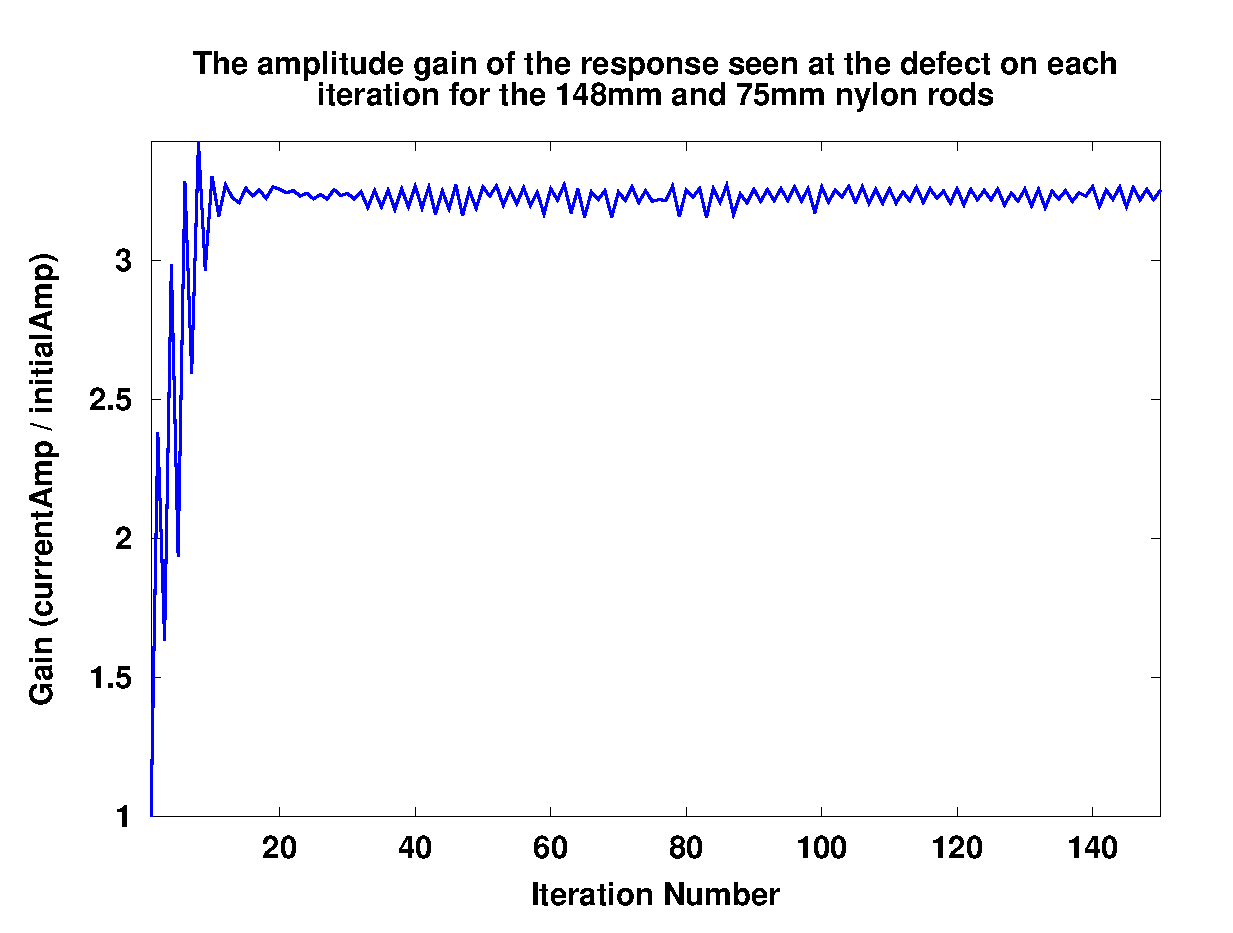
\includegraphics[width=0.6\textwidth]{eps_pics/nylon-2-4_iterationVsGain.eps}
 \caption{Defect amplitude gain that was achieved at the defect for each iteration of the time reversal algorithm for the $148 mm$ and $75 mm$ nylon rods. The final gain of a little over 3 was reached by about the 25th iteration as seen in other tests.
  	 \label{fig:nylonIter2}} 
 \end{figure}
 
 \begin{figure}[ht!]
 \centering
 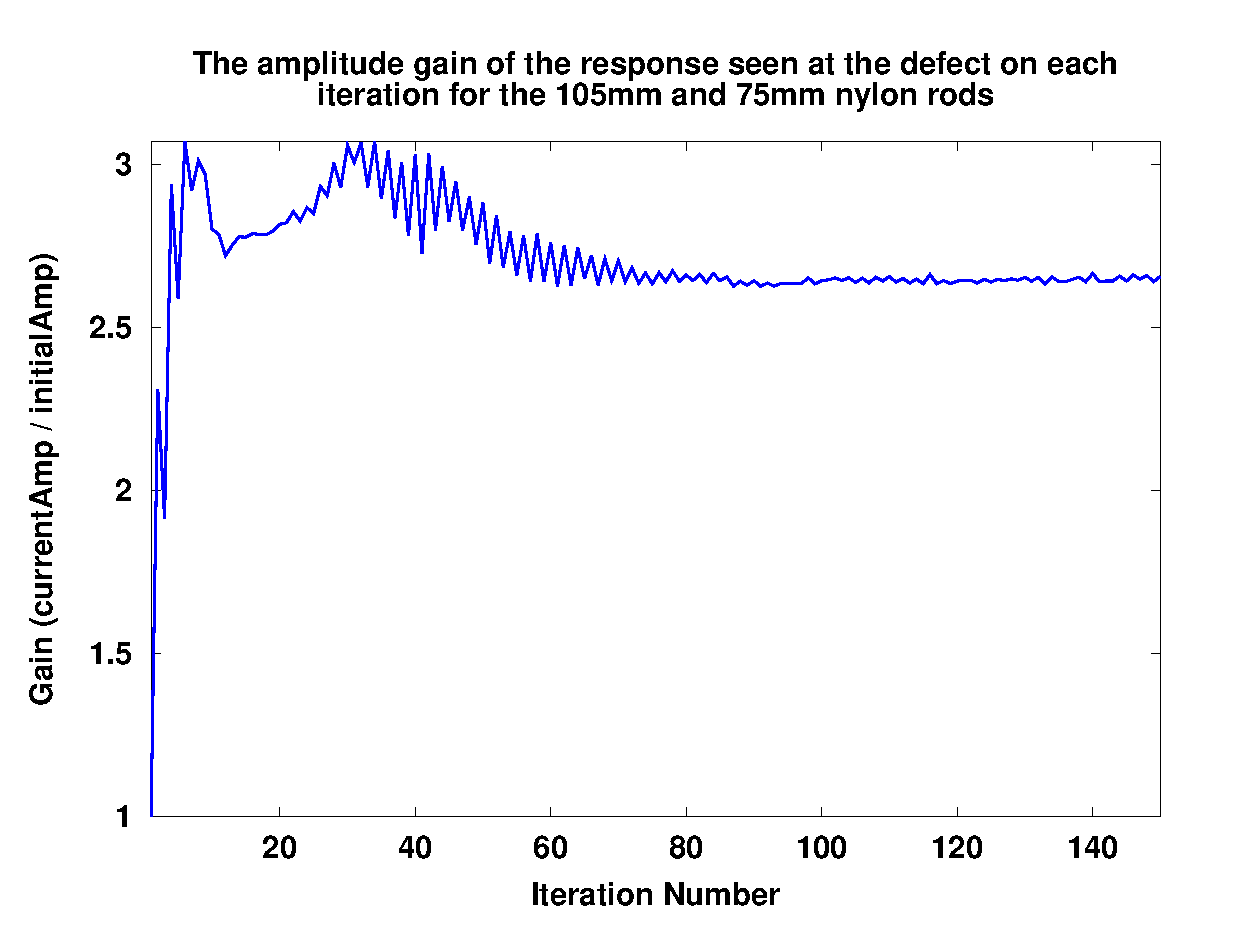
\includegraphics[width=0.6\textwidth]{eps_pics/nylon-3-4_iterationVsGain.eps}
 \caption{Defect amplitude gain that was achieved at the defect for each iteration of the time reversal algorithm for the $105 mm$ and $75 mm$ nylon rods. The final gain seen was about 2.75. This test was a good example of the final gain being lower than the max gain that was seen and suggests that the algorithm could be further improved.
  	 \label{fig:nylonIter3}} 
 \end{figure}
 
 
  \begin{figure}
 \begin{subfigmatrix}{2}
 \subfigure[Defect Response Initial Iteration, $148 mm$ and $105 mm$ nylon rods]
 {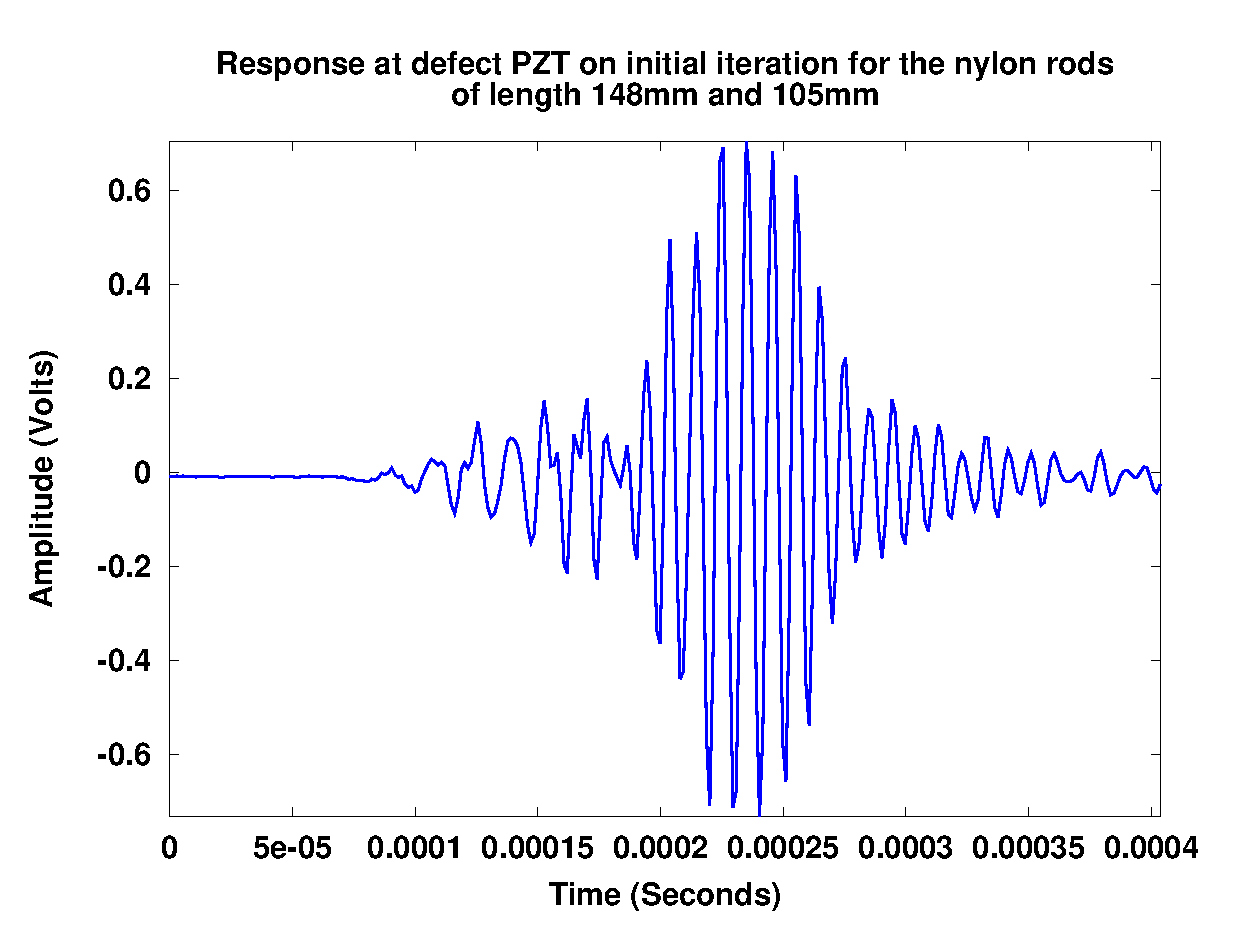
\includegraphics[width=0.6\textwidth]{eps_pics/nylon-2-3_Initial.eps}}
 \subfigure[Defect Response 150th Iteration, $148 mm$ and $105 mm$ nylon rods]
 {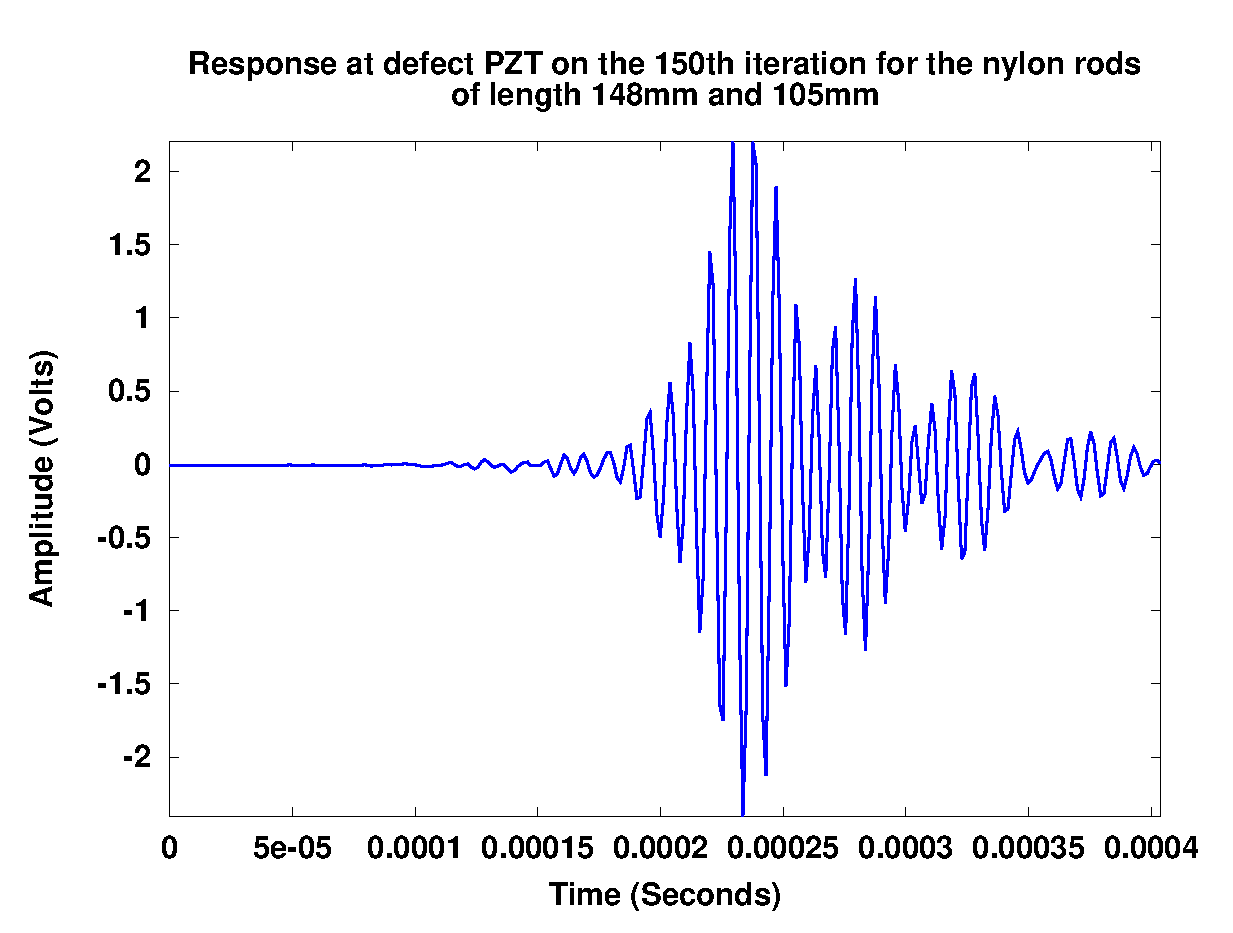
\includegraphics[width=0.6\textwidth]{eps_pics/nylon-2-3_Final.eps}}
 \end{subfigmatrix}
 
    \caption
 %>>>> use \label inside caption to get Fig. number with \ref{}
    { \label{fig:nylonExp1}
    a) First wave seen at the defect on the initial iteration for the $148 mm$ and $105 mm$ nylon rod test.; b) Wave recorded at the defect after 150 iterations. The final wave more than tripled in amplitude from the first wave.
  }
 \end{figure}
 
  \begin{figure}
 \begin{subfigmatrix}{2}
 \subfigure[Defect Response Initial Iteration, $148 mm$ and $75 mm$ nylon rods]
 {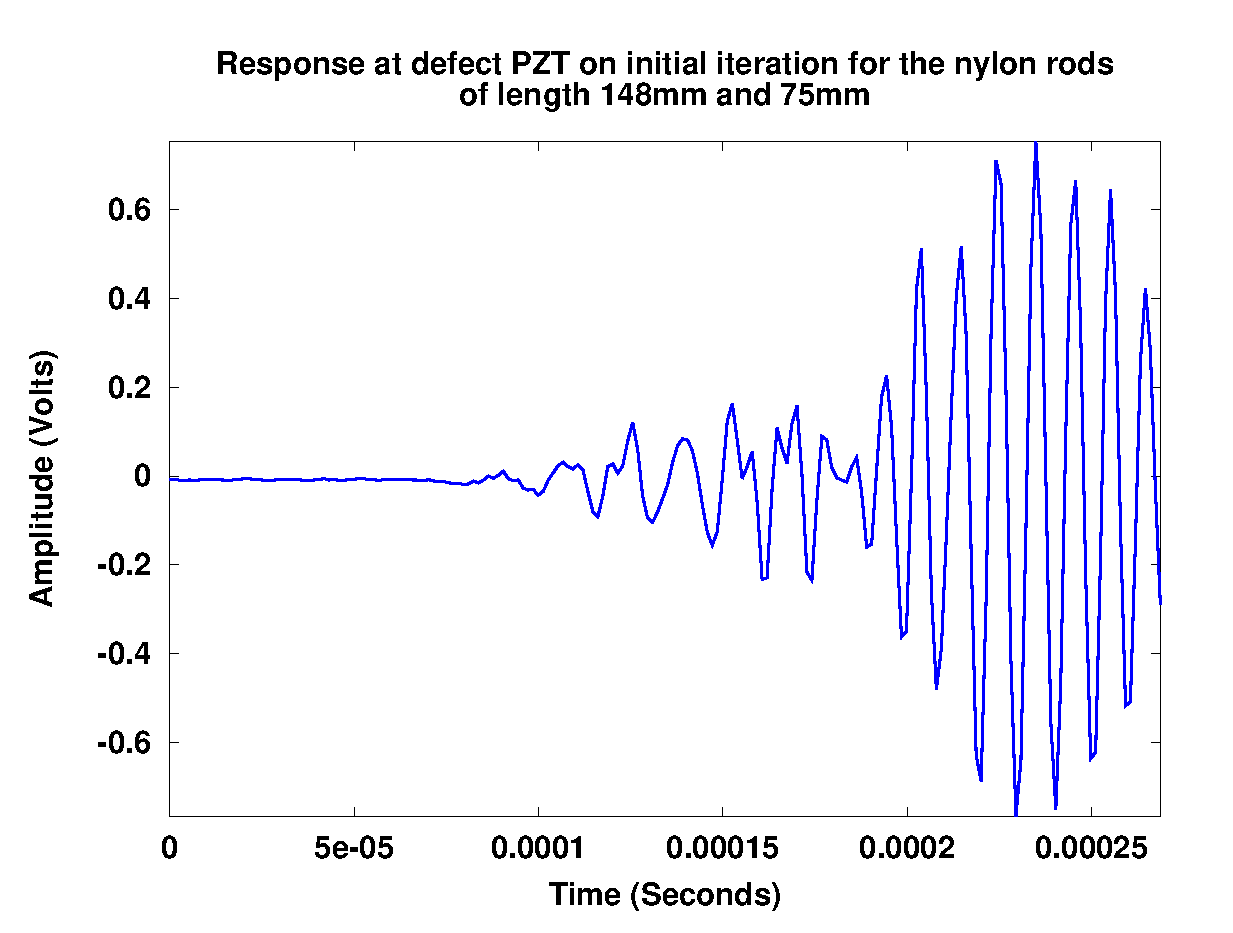
\includegraphics[width=0.6\textwidth]{eps_pics/nylon-2-4_Initial.eps}}
 \subfigure[Defect Response 150th Iteration, $148 mm$ and $75 mm$ nylon rods]
 {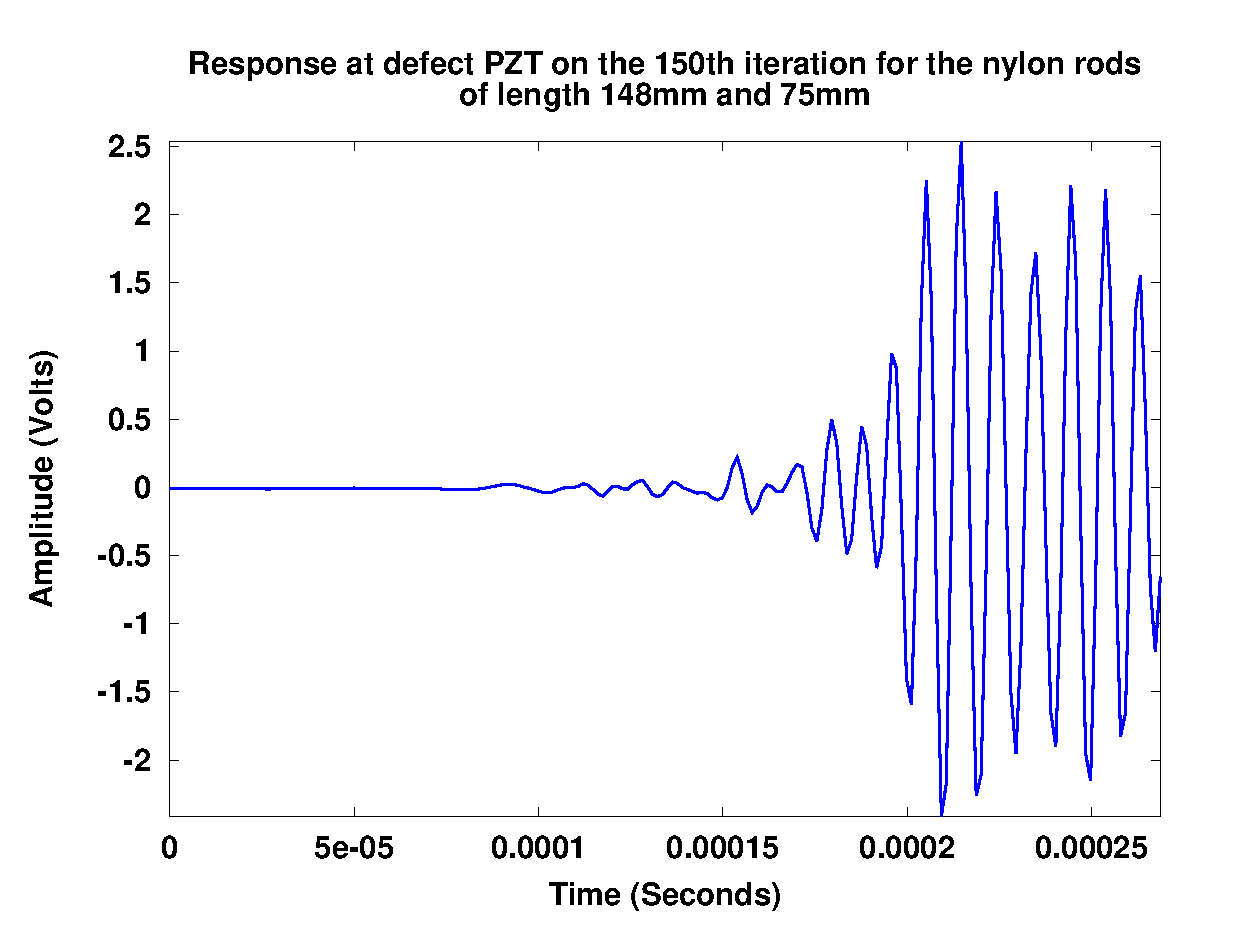
\includegraphics[width=0.6\textwidth]{eps_pics/nylon-2-4_Final.eps}}
 \end{subfigmatrix}

    \caption
 %>>>> use \label inside caption to get Fig. number with \ref{}
    { \label{fig:nylonExp2}
    a) First wave seen at the defect on the initial iteration for the $148 mm$ and $75 mm$ nylon rod test.; b) Wave recorded at the defect after 150 iterations. Again, the response seen at the defect has tripled.
  }
 \end{figure}
 
  \begin{figure}
 \begin{subfigmatrix}{2}
 \subfigure[Defect Response Initial Iteration, $105 mm$ and $75 mm$ nylon rods]
 {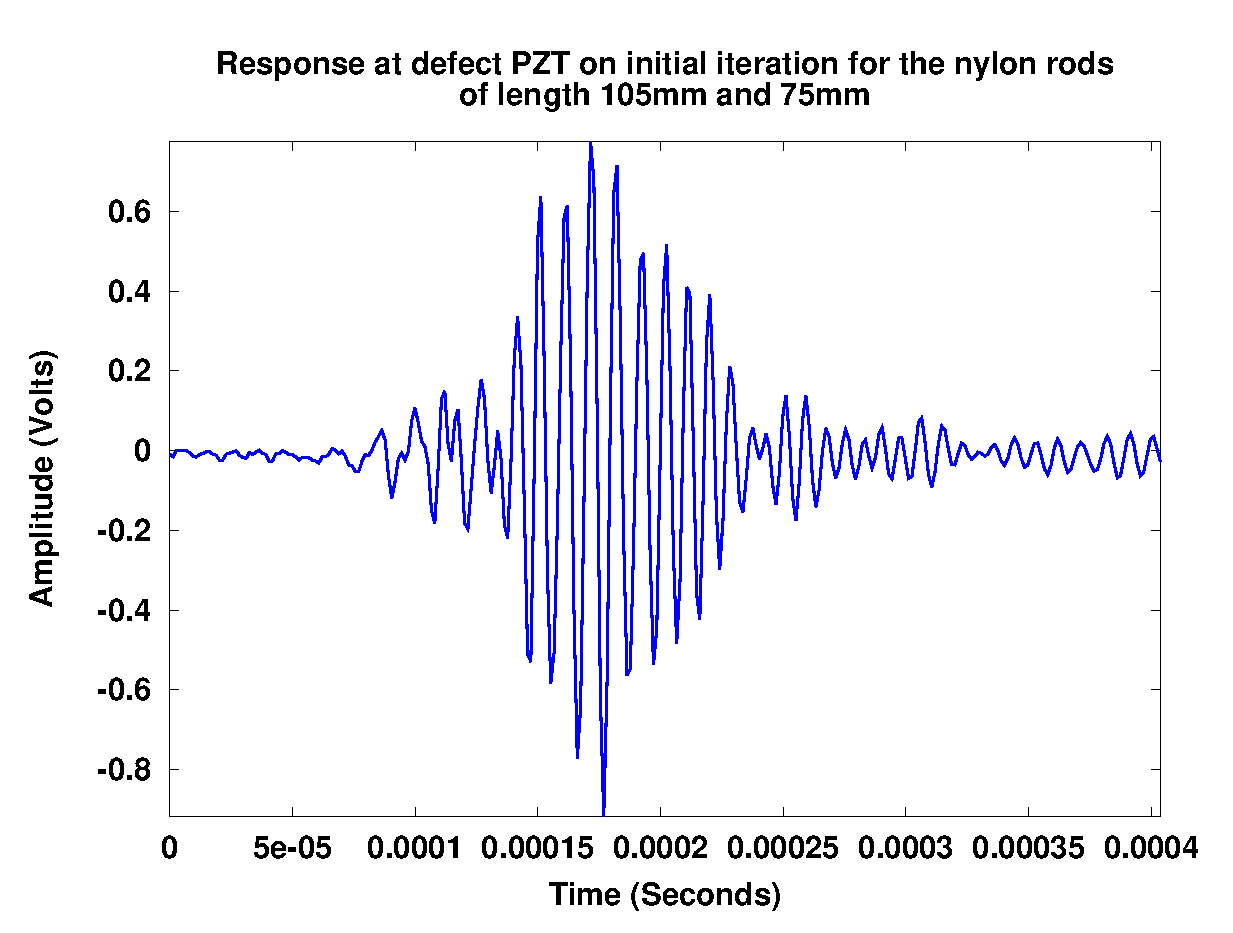
\includegraphics[width=0.6\textwidth]{eps_pics/nylon-3-4_Initial.eps}}
 \subfigure[Defect Response 150th Iteration, $105 mm$ and $75 mm$ nylon rods]
 {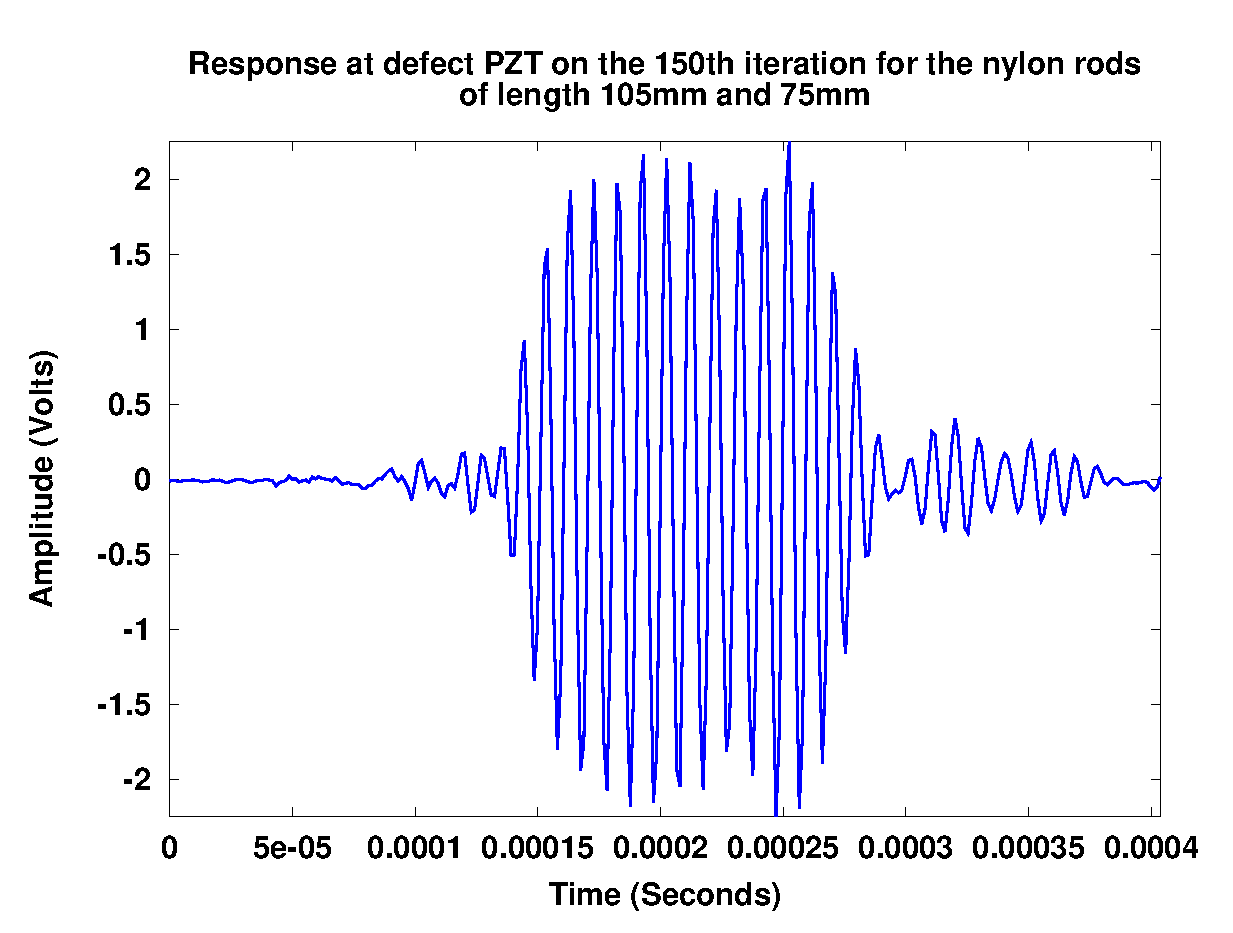
\includegraphics[width=0.6\textwidth]{eps_pics/nylon-3-4_Final.eps}}
 \end{subfigmatrix}
 
    \caption
 %>>>> use \label inside caption to get Fig. number with \ref{}
    { \label{fig:nylonExp3}
    a) First wave seen at the defect on the initial iteration for the $105 mm$ and $75 mm$ nylon rod test.; b) Wave recorded at the defect after 150 iterations.
  }
 \end{figure}
 